% !TEX program = xelatex
% =====================================================================
%  flico 研究日誌 (research log) 主檔
%
%  編譯指令:
%    xelatex log.tex && biber log && xelatex log.tex && xelatex log.tex
%  (或 latexmk -xelatex log)
%
%  寫日誌的方式:
%    1. 在 entries/ 下新增一個檔 YYYY-MM-DD.tex(每日一檔)
%    2. 若該日有圖,把圖放在 figures/YYYY-MM-DD/ 下
%    3. 在本檔最下方的「日誌條目」區塊追加兩行:
%         \section{YYYY-MM-DD —— 標題}
%         \input{entries/YYYY-MM-DD}
%    4. 重新編譯。
%
%  preamble 與 report/main.tex 共用同一套中文排版設定。
% =====================================================================
\documentclass[12pt,a4paper]{article}

% ---- 版面 ----------------------------------------------------------
\usepackage[margin=1in]{geometry}
\usepackage{setspace}
\onehalfspacing
\usepackage{titling}
\setlength{\droptitle}{-1.5cm}
\usepackage{fancyhdr}
\setlength{\headheight}{15pt}
\pagestyle{fancy}\fancyhf{}
\renewcommand{\headrulewidth}{0.4pt}
\lhead{\leftmark}\rhead{\thepage}
\parindent=24pt

% ---- 數學與符號 ----------------------------------------------------
\usepackage{amsmath,amsthm,amssymb,amsbsy,bm}
\usepackage{siunitx}

% ---- 圖、表 --------------------------------------------------------
\usepackage{graphicx}
\graphicspath{{figures/}}
\usepackage{float}
\usepackage{subfig}
\usepackage{booktabs}
\usepackage{array}
\usepackage{multirow}
\usepackage{longtable}
\usepackage{enumitem}

% ---- 連結 ----------------------------------------------------------
\usepackage{xcolor}
\usepackage[unicode=true,pdfborder={0 0 0},bookmarksdepth=-1,
            colorlinks=true,linkcolor=blue!55!black,citecolor=blue!55!black,
            urlcolor=teal]{hyperref}

% ---- 參考文獻(biblatex + biber)----------------------------------
\usepackage[backend=biber,style=numeric,giveninits=true]{biblatex}
\addbibresource{references.bib}

% ---- 中文字型:TW-Kai,並啟用「假粗體 / 假斜體」-------------------
\usepackage{xeCJK}
\setCJKmainfont{TW-Kai}[AutoFakeBold=2.5, AutoFakeSlant=0.2]
\setCJKmonofont{TW-Kai}[AutoFakeBold=2.5, AutoFakeSlant=0.2]
\setCJKsansfont{TW-Kai}[AutoFakeBold=2.5, AutoFakeSlant=0.2]

% ---- 自訂指令 / 環境 -----------------------------------------------
\newcommand{\gauss}{\ \text{G}}
% 「日誌條目」section 的格式微調:不縮排、上方多留空白以便目視分隔
\newcommand{\logentry}[2]{%
  \clearpage
  \section[#1 —— #2]{\texorpdfstring{#1\quad #2}{#1 — #2}}%
}

% =====================================================================
\title{\bfseries flico 研究日誌\\[4pt]
       \large flicker meter \(=\) BPW34 \(+\) MCP6004 TIA \(+\) Raspberry Pi Pico}
\author{Polarbear\\ \normalsize 國立臺灣大學}
\date{起始於 2026 年 6 月 2 日}

\begin{document}
\maketitle
\thispagestyle{fancy}
\tableofcontents
\clearpage

% =====================================================================
%  日誌條目 (entries) — 新增日誌時在下面 append \logentry + \input
% =====================================================================

\logentry{2026-04-19}{構想階段:從分壓電阻到 TIA、DC/AC 雙模四檔光學量測儀提案}
% =====================================================================
%  2026-04-19 — 構想階段:從分壓電阻到 TIA、DC/AC 雙模四檔光學量測儀提案
% =====================================================================

\subsection*{緣起與初始想法}

想做一台可以同時測「螢幕更新率」與「螢幕亮度」的小儀器。腦中先冒出的訊號鏈如下:

\begin{quote}
給光二極體 (PD) 一個逆偏壓,串一顆電阻把分壓墊高,再用電容把 DC 濾掉,
之後用取樣頻率夠高的 ADC 把電壓訊號轉成數位訊號,送到電腦做傅立葉。
\end{quote}

物理直覺:光電流 \(I_p \propto\) 入射光功率;入射光功率本身是「環境亮度 (DC)」與
「螢幕刷新/PWM 調光擾動 (AC)」的疊加。AC 用 FFT 抓峰、DC 用平均換亮度,
兩件事一支感測器同時做。

\subsection*{被導正的關鍵點:從分壓電阻到 TIA}

跟 Gemini 對談時被點出:純串聯負載電阻有
\textbf{增益-頻寬權衡 (Gain-Bandwidth Trade-off)}。
PD 自帶接面電容 \(C_j\)。為了把微弱光電流放大成有用電壓,
\(R_L\) 通常會選得大,但 \(R_L\) 與 \(C_j\) 會構成一個 RC 低通,
截止頻率
\begin{equation}
  f_c \;=\; \frac{1}{2\pi R_L C_j}.
  \label{eq:0503-fc}
\end{equation}
若我把 \(R_L\) 設到 \(\SI{1}{\mega\ohm}\)、PD 是 BPW34
(零偏壓下 \(C_j \approx \SI{72}{\pico\farad}\)),
代入式~\eqref{eq:0503-fc} 得 \(f_c \approx \SI{2.2}{\kilo\hertz}\) ——
這把要量的 OLED PWM (\(\sim \SI{480}{\hertz}\) 以上的諧波)
與部分螢幕刷新諧波都吃掉了。\textbf{要嘛犧牲增益、要嘛犧牲頻寬,無解。}

解法:改用\textbf{轉阻放大器 (Transimpedance Amplifier, TIA)}。
把 PD 接在運算放大器的反相輸入端,反相端被虛地 (Virtual Ground) 固定住,
\(C_j\) 兩端電壓不再變動,RC 延遲就不再決定頻寬,可以同時做到「高增益」與「高頻寬」,
方波邊緣也才會夠陡。輸出電壓
\begin{equation}
  V_\text{out} \;=\; I_p \, R_F .
  \label{eq:0503-tia}
\end{equation}
這個觀念上的轉變是今天最大的收穫:從「分壓電路」改成「跨阻電路」之後,
我們的設計空間突然開闊很多。

\subsection*{量測目標與動機}

具體想驗證四件事:

\begin{itemize}[leftmargin=2em,itemsep=0pt]
  \item \textbf{市電 \(\SI{60}{\hertz}\) 照明閃爍} —— 家用 AC 燈泡應該會有 \(\SI{60}{\hertz}\)
        (亮度上的能量主要在二次諧波 \(\SI{120}{\hertz}\)) 的閃爍,
        看看實際量得到嗎?
  \item \textbf{Apple ProMotion 變動更新率} —— iPhone 13/14 Pro 最低 \(\SI{10}{\hertz}\)、
        15 Pro 可降到 \(\SI{1}{\hertz}\)。LTPO 真的會動嗎?能不能被光學側量到?
  \item \textbf{OLED PWM 調光} —— 常見頻率落在 \(\SI{240}{\hertz}\) 到 \(\SI{480}{\hertz}\),
        是否低到讓眼睛不舒服?
  \item \textbf{螢幕峰值亮度} —— 各家 HDR 標稱的 \(\si{\candela\per\square\metre}\)
        是真有那麼亮、還是只是行銷數字?
\end{itemize}

\subsection*{裝置構想 (提案摘要)}

依上面的目標,構想一台口袋型儀器:

\begin{itemize}[leftmargin=2em,itemsep=0pt]
  \item \textbf{雙模式}:用一顆撥動開關切 \textbf{DC mode}(讀亮度) 與
        \textbf{AC mode}(送 FFT 抓頻率)。
  \item \textbf{四檔增益旋鈕}:轉動波段開關切換 TIA 的回授電阻 \(R_F\)
        (例如 \(\SI{10}{\kilo\ohm}\) / \(\SI{100}{\kilo\ohm}\) /
        \(\SI{1}{\mega\ohm}\) / 預留一檔),
        以覆蓋從強光到弱光的大動態範圍。
  \item \textbf{顯示}:4 位數 7 段顯示器 (TM1637),即時顯示亮度或 FFT 峰值頻率。
  \item \textbf{電源}:\(\SI{3.7}{\volt}\) 鋰聚合物電池 + TP4056 Type-C 充電 +
        LDO 穩壓到 \(\SI{3.3}{\volt}\)。
  \item \textbf{尺寸目標}:\(< \SI{50}{\milli\metre}\!\times\!\SI{50}{\milli\metre}
        \!\times\!\SI{30}{\milli\metre}\),單手貼螢幕可量。
\end{itemize}

系統方塊圖(訊號鏈):

\begin{verbatim}
  [待測光源]
        |
        v
  [Photodiode]----->[TIA + Rf 旋鈕切換增益]
                                 |
                +----------------+----------------+
                v                                 v
        [DC: LPF 取平均]              [AC: 耦合電容 + Vref 偏壓 ~1.65V]
                |                                 |
                +-------> [MCU ADC] <-------------+
                              |
                              v
                       [DC 平均 / AC FFT]
                              |
                              v
                  [4 位 7 段顯示器 (TM1637)]
\end{verbatim}

\subsection*{初步電路設計重點}

\begin{itemize}[leftmargin=2em,itemsep=0pt]
  \item \textbf{TIA 回授}:\(R_F\) 與一顆補償電容 \(C_F\)
        (\(\SI{10}{\pico\farad}\) 量級) 並聯,壓制 \(C_j\) 引起的高頻震盪。
  \item \textbf{雙路訊號分離}:TIA 輸出分兩路 —— 一路 LPF (\(f_c \lesssim \SI{10}{\hertz}\))
        取 DC 亮度;另一路 AC 耦合 + 用兩顆等值電阻分壓做
        \(V_\text{ref} = V_\text{DD}/2 \approx \SI{1.65}{\volt}\) 偏置,
        把 AC 訊號中心墊到 MCU ADC 可讀的正電壓區。
  \item \textbf{AC 路高通的低頻極限}:要量到 ProMotion 的 \(\SI{1}{\hertz}\),
        高通截止得遠低於 \(\SI{1}{\hertz}\) (例如 \(\SI{0.1}{\hertz}\)),
        所以耦合電容 \(\times\) 後級阻抗的 \(\tau\) 要做大。
  \item \textbf{抗混疊}:ADC 取樣率規劃 \(f_s = \SI{5}{}\sim\SI{10}{\kilo\hertz}\),
        進 ADC 前加一階 RC LPF,\(f_c \approx f_s/2\),
        避免 \(>f_s/2\) 的雜訊摺回打到 PWM 譜峰。
\end{itemize}

\subsection*{初步 BOM 與時程}

對話中已經整理出八節提案 (動機 / 原理 / 電路 / 規格 / 外觀 / BOM / 時程 / 結語)。
細節留在提案書本身,日誌只記重點:

\begin{itemize}[leftmargin=2em,itemsep=0pt]
  \item BOM:總價估 \(\textbf{TWD 580--680}\),
        台灣本地 (光華商場、Mouser/Digi-Key 台灣站、蝦皮) 都能備齊。
  \item 時程:\textbf{8 週} —— 第 1 週採購與環境;2--3 週麵包板原型 (TIA 調 \(R_F\)、\(C_F\));
        4 週 ADC + DMA;5 週 FFT;6 週顯示器/旋鈕/開關整合;
        7 週焊板 / 進外殼;8 週校準與結案。
\end{itemize}

\subsection*{今日尚未拍板的選擇}

\begin{itemize}[leftmargin=2em,itemsep=0pt]
  \item \textbf{Op-amp}:暫定 \texttt{TL072} 或 \texttt{MCP6002} 二擇一。
        TL072 是雙電源音響元件、單 \(\SI{3.3}{\volt}\) 不能用,
        應該會傾向 \textbf{MCP6002} (Rail-to-Rail、CMOS、低偏壓電流),
        但要再確認 datasheet。
  \item \textbf{Photodiode}:暫記 \textbf{BPW34}。但 BPW34 譜響應峰值在
        \(\SI{920}{\nano\metre}\) (近紅外),與人眼 \(V_\lambda\)
        峰值 \(\SI{555}{\nano\metre}\) 嚴重不合,測「亮度」會失真。
        下一步要找帶 \(V_\lambda\) 濾波的 PD,或在感光窗前加 IR-Cut。
  \item \textbf{MCU}:STM32 系列;但對「跑得動 FFT 又便宜小巧」這個 axis 上,
        Raspberry Pi Pico (RP2040, \(\SI{133}{\mega\hertz}\) M0+, \(\SI{264}{\kilo\byte}\)
        RAM) 也是熱門選項。下次再評估。
  \item \textbf{旋鈕}:純機械的波段開關手感好但有「先斷後接」的瞬間突波;
        類比開關 IC (例如 TMUX1104) 由 MCU 控制可以避開機械抖動。
        要不要為了極致小型化改 IC 切換,日後決定。
\end{itemize}

\subsection*{今日心得}

\begin{itemize}[leftmargin=2em,itemsep=0pt]
  \item 最大收穫是觀念:原本以為「分壓 + 高速 ADC」就夠了,
        其實 \(R_L C_j\) 那個低通會把 PWM 高頻砍掉。
        TIA 的虛地直接把 \(C_j\) 對頻寬的影響拿掉,這個 trick 必記。
  \item 「DC 模式」與「AC 模式」其實是同一個 TIA 後面接兩條 path 的問題,
        不是兩個獨立電路;旋鈕切的是 \(R_F\),不是切模式。模式由開關控制,
        旋鈕控的是動態範圍。
  \item 單電源 \(\SI{3.3}{\volt}\) 系統不能直接吃 LiPo
        (滿電 \(\SI{4.2}{\volt}\) 會燒 MCU),必須加 LDO。
        這件事不能在 BOM 上漏掉。
  \item 下一步 (5/4--):查 BPW34 vs SFH-2440 譜匹配、敲定 op-amp 型號、
        把提案書整理乾淨給老師看。
\end{itemize}


\logentry{2026-04-21}{第一次去光華:今華電子採購記}
% =====================================================================
%  2026-04-21 — 第一次去光華:今華電子採購記
% =====================================================================

\subsection*{今日目標}

\begin{itemize}[leftmargin=2em,itemsep=0pt]
  \item 帶著 4/19 跟 Gemini 對話整理出來的「必買 / 可以等 / 實驗室借用」三張清單,
        到光華商場地下室實地採買,把麵包板實驗的零件補齊。
  \item 走「無烙鐵」路線:這次只湊到能在麵包板上插出類比前端 TIA 的東西,
        STM32 排針焊接、SFH 2440、烙鐵都留給網購。
  \item 用 Gemini chat 當「邊走邊問的店內顧問」,遇到老闆指著我看不懂的東西、
        或是貨架上 MCP6002 缺貨時即時備援。
\end{itemize}

\subsection*{地點 \& 時間}

\textbf{今華電子有限公司台北分公司}(北市新生南路一段 12 巷 2 號,TEL: 02-23921111),
2026-04-21 (一) 13:41 結帳。光華地下室,離源達科技不遠。

\subsection*{邊買邊問:Gemini 在現場救了哪些急?}

實際逛貨架時,清單上的東西不是每樣都長得跟想像中一樣,
這時候用手機拍照丟給 Gemini 確認非常有用。今天用上的幾個臨場提問:

\begin{itemize}[leftmargin=2em,itemsep=0pt]
  \item \textbf{「這個可以當作 TM1637 嗎?」} —— 包裝寫「4 位數時鐘顯示模組」
        沒寫 TM1637,Gemini 教我隔著塑膠袋找 \texttt{VCC/GND/DIO/CLK} 四根排針,
        確認就是同一顆。OK,放進籃子。
  \item \textbf{「\(\,\)EIC-1104 / 1106 / 1108 哪一塊比較適合?」} —— 老闆櫃台同時擺了三個尺寸。
        Gemini 推 1104:雙區設計可做「類比區 / 數位區」分離,1106/1108 太大佔桌面,
        對螢幕貼近量測反而不方便。
  \item \textbf{「\(\,\)EIC-1104 還需要 MB102 嗎?」} —— EIC-1104 帶接線柱,看起來像高級電源板,
        但其實它只是「馬路」,不會自己發電。沒實驗室的大電供時,必買 MB102 給 5 V 轉 3.3 V。
  \item \textbf{「BPW34 又會叫什麼名字?」} —— 怕老闆聽不懂型號,Gemini 教我退而求其次叫
        「光敏二極體」、「平頭的接收管」、或「矽光電池」。實際上今華有原裝 Vishay BPW34,
        所以這招沒用上,但學起來。
  \item \textbf{「\(\,\)Pico PR2040 可以嗎?」} —— 我把 RP2040 跟 Pico 搞混,Gemini 解釋
        RP2040 就是 Pico 上面那顆晶片;Pico 板就是 RP2040 + 周邊。我要的是那塊板。
  \item \textbf{「沒有 MCP6002 還有哪些放大器可以選擇呢?」} —— **這是今天最痛的一題**。
        架上沒 MCP6002,Gemini 提了 LMC6482、MCP6022、TLC2272 三個 DIP-8 替代品,
        又警告 LM358 / TL072 / NE5532 是地雷不能拿。最後\textbf{今天店裡這幾顆都沒有貨},
        op-amp 空手而回(詳見下面「漏買」一節)。
  \item \textbf{「那 MCP6008 可以嗎?」} —— 看貨架瞄到一個型號像的 IC,問了 Gemini 才知道
        MCP6008 根本不存在;我可能跟 MCP3008 (那是 8 通道 ADC) 或 MCP608 搞混。差點買錯。
  \item \textbf{「DC 圓頭哪一根是正極?」} —— 拿到「9V 電池扣轉 DC 公頭」轉接頭,兩根金屬針沒標示。
        Gemini 教我用三用電表蜂鳴檔測導通,找出哪根通到中心、哪根通到外圈,然後遵循 MB102 的
        「\textbf{內正外負}」(Center Positive)規範。
\end{itemize}

\subsection*{購買清單與收據}

最後刷掉 \(\textbf{TWD 1{,}530}\) 現金,收據如圖~\ref{fig:0421-receipt}。

\begin{figure}[H]
  \centering
  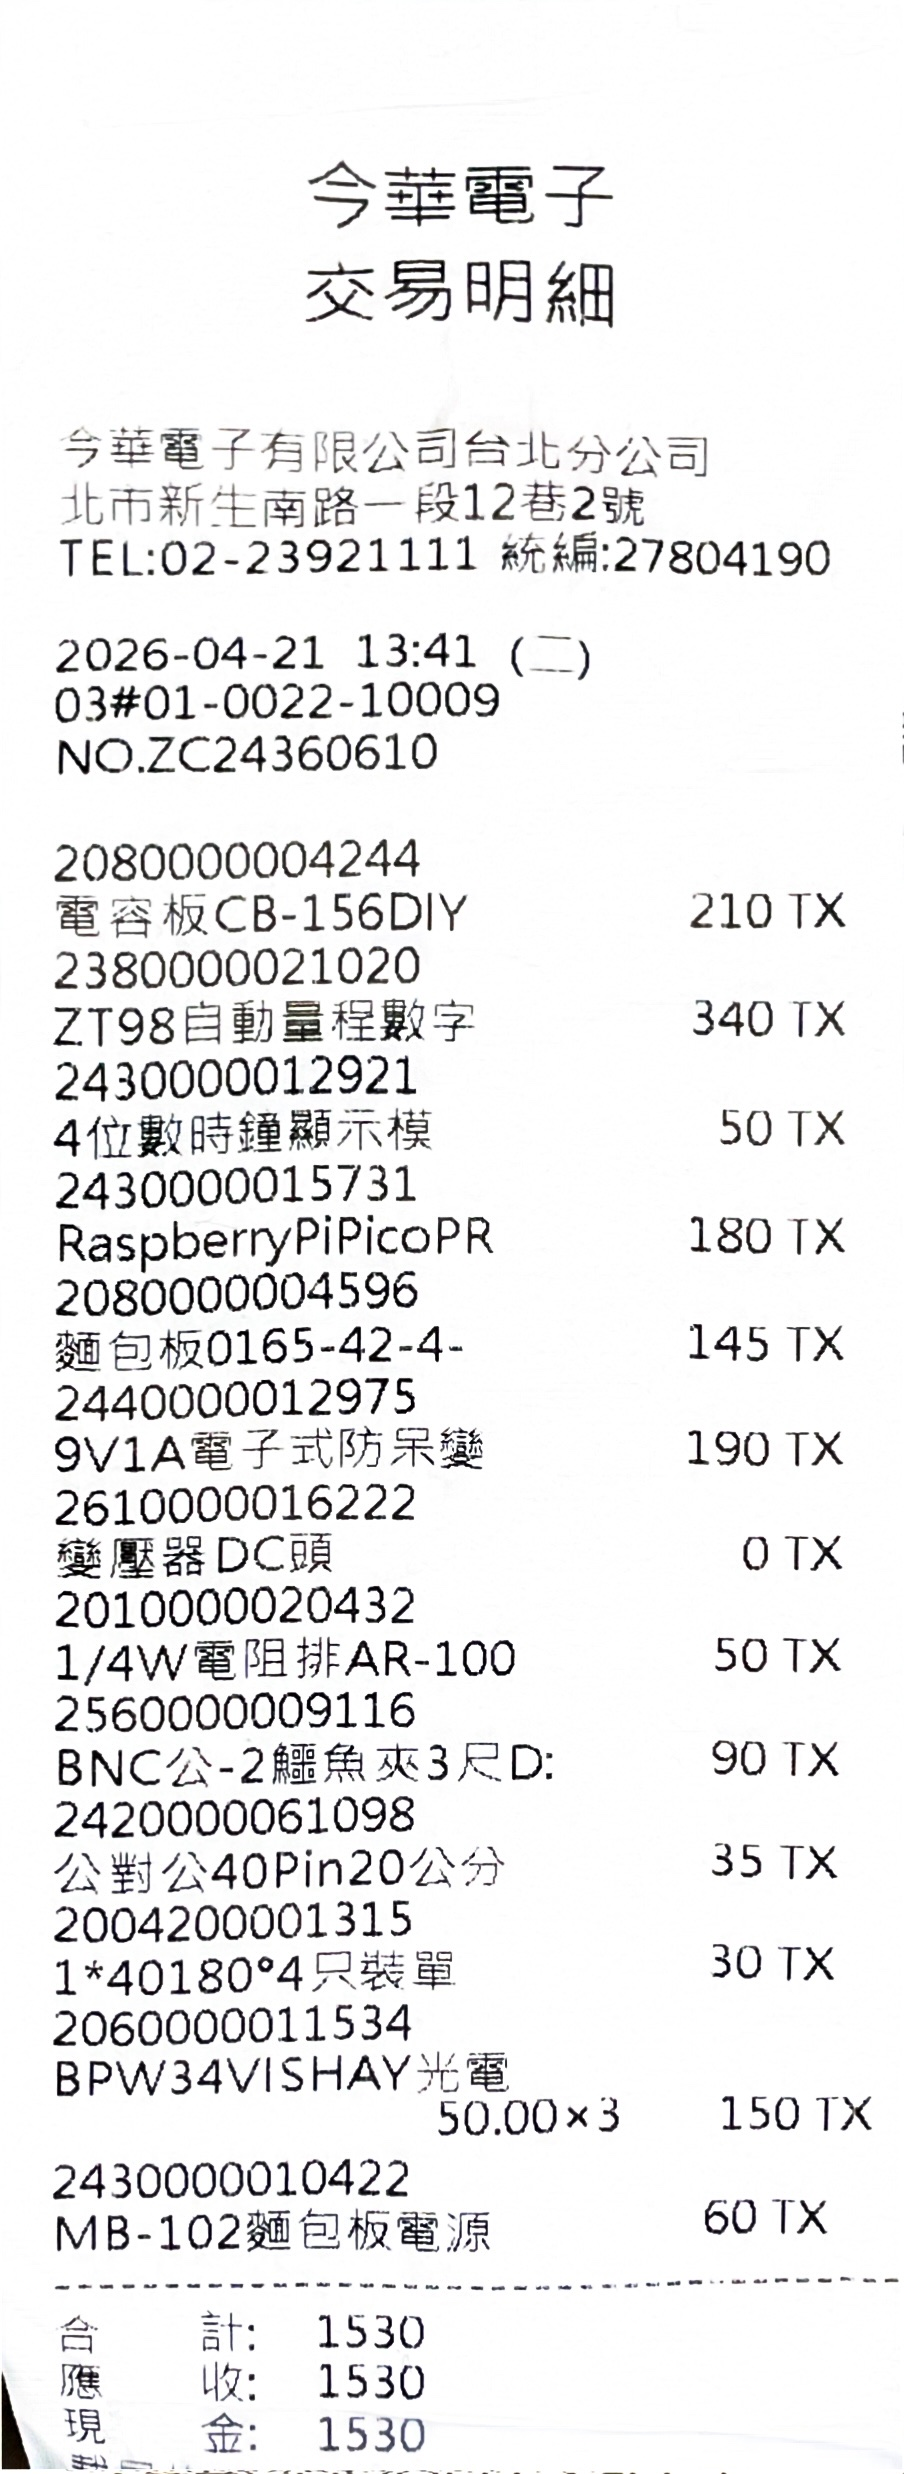
\includegraphics[width=0.55\linewidth]{2026-04-21/今華電子交易明細0421.jpg}
  \caption{今華電子 2026-04-21 13:41 交易明細,合計 TWD 1530。}
  \label{fig:0421-receipt}
\end{figure}

明細整理:

\begin{table}[H]
  \centering
  \caption{4/21 今華電子採購明細。}
  \label{tab:0421-bom}
  \begin{tabular}{llrr}
    \toprule
    類別 & 品項 & 數量 & 小計 (TWD) \\
    \midrule
    儀器 & ZT98 自動量程數位三用電表          & 1 & 340 \\
    平台 & EIC-1104 等級麵包板 (型號 0165-42-4-)  & 1 & 145 \\
    電源 & MB-102 麵包板電源模組               & 1 & 60  \\
    電源 & 9V / 1A 電子式防呆變壓器             & 1 & 190 \\
    電源 & 變壓器 DC 頭(9V 電池扣轉接)         & 1 & 0   \\
    MCU  & Raspberry Pi Pico (RP2040, Type-C 版) & 1 & 180 \\
    顯示 & TM1637 4 位 7 段顯示模組             & 1 & 50  \\
    感測 & Vishay BPW34 光電二極體              & 3 & 150 \\
    被動 & 電容板 CB-156 DIY 電容組合包         & 1 & 210 \\
    被動 & 1/4 W 色碼電阻排 AR-100              & 1 & 50  \\
    接線 & 公對公 40-pin 20 cm 杜邦線            & 1 & 35  \\
    接線 & 1$\times$40 180° 單排排針(4 入裝)    & 1 & 30  \\
    量測 & BNC 公頭轉 2 鱷魚夾線,3 ft            & 1 & 90  \\
    \midrule
    \multicolumn{3}{r}{\textbf{合計(現金)}} & \textbf{1{,}530} \\
    \bottomrule
  \end{tabular}
\end{table}

幾個現場決定的細節:

\begin{itemize}[leftmargin=2em,itemsep=0pt]
  \item \textbf{BPW34 買 3 顆}是備援 —— 第一次接 TIA 很容易接反極性或燒掉,150 元便宜保險。
  \item \textbf{電容板 CB-156 DIY} 是臨時加碼。Gemini 原本只要求 10 pF、22 pF、104 各幾顆,
        但老闆推這盒 156 種規格全包,210 元划算,以後不會缺電容值,
        後面要調補償電容也比較有彈性。
  \item \textbf{9V/1A 變壓器 + DC 頭}是 Gemini 提醒的「容易忽略的致命細節」:
        MB-102 的圓孔必須吃 7--12 V 輸入,USB 5 V 不夠。沒這條線今天就白跑了。
  \item \textbf{BNC--鱷魚夾線 90 元}是預先為後續實驗室示波器架設準備的;
        系上實驗室通常只給 BNC 介面,沒這條線連不上麵包板。
\end{itemize}

\subsection*{走到源達補貨:MCP6004 \(\times\,\)2}

今華結帳後,因為 op-amp 整批缺貨,直接走去隔壁的\textbf{源達科技}補。源達櫃台
剛好有 \textbf{MCP6004}(DIP-14,內含 4 顆 op-amp),雖然 Gemini 提醒 MCP6004
是「14 根腳的大蜈蚣、未用的 op-amp 要接成 voltage follower 否則高頻干擾」,
但內部規格跟 MCP6002 一模一樣,接腳 100\% 相容專題需求,當下就拿了。

\textbf{兩顆 MCP6004,單價忘記了,暫記每顆 50,合計 100 TWD(等發票補齊)}。
這樣專題靈魂的類比核心元件總算到手,類比前端 TIA 接下來就可以開工。

\subsection*{今天還沒買的東西(留給網購)}

\begin{itemize}[leftmargin=2em,itemsep=0pt]
  \item \textbf{波段開關(增益旋鈕)\& 撥動開關(AC/DC 模式)} —— 今華有貨但決定暫緩。
        Gemini 提醒過機械波段開關接腳粗,直插麵包板會撐壞簧片;
        先用「手動拔線換 \(R_F\)」模擬切檔就好,等真的進外殼再買。
  \item \textbf{烙鐵 / 焊錫 / SFH 2440 / SMD 轉 DIP 轉接板 / 3.7 V LiPo / TP4056 / LDO} ——
        全列為「可以等(網購)」,今天不買。
\end{itemize}

\subsection*{今日實驗進度}

回家拆完戰利品,只跑到「電源軌通電」這一步就收工:

\begin{enumerate}[leftmargin=2em,itemsep=2pt]
  \item 把 9 V/1 A 變壓器跟 DC 公頭轉接頭組裝起來。先用三用電表蜂鳴檔確認轉接頭中心極對應的金屬針,
        把變壓器的線接到中心極 (+),外圈那根接外圈 (-)。
  \item 上電前最後 double check:三用電表轉到 DC V,紅探針進中心孔、黑探針碰外圈,
        讀到 \textbf{+9.0 V},極性沒接反。
  \item 把轉接頭插進 MB-102 的 5.5$\times$2.1 mm 圓孔,MB-102 上的小撥桿撥到 3.3 V 檔位。
  \item 把 MB-102 跨插到 EIC-1104 麵包板的電源軌上。
  \item 用三用電表量麵包板紅軌跟藍軌之間的電壓,讀到 \textbf{\(\sim\)3.30 V 直流},
        電源軌通電成功。
\end{enumerate}

\textbf{今天就停在這。}沒接 op-amp、沒接 PD、沒進 TIA 階段 —— 因為今華沒 op-amp 的時候我已經
逛累了,源達補完 MCP6004 拿回家天已經黑;先把電源接通、確認沒短路冒煙,
等明天再開始照 Gemini 給的步驟接 TIA。

\subsection*{今日心得}

\begin{itemize}[leftmargin=2em,itemsep=0pt]
  \item 第一次去光華,最大收穫不是材料,而是學會\textbf{「邊走邊問」的工作流}:
        把 Gemini 當駐店顧問,拍照確認模組、問替代品、問封裝差異 ——
        現場決策品質會高很多。
  \item 跟老闆對話得用對術語:\textbf{DIP-8 vs SMD}、\textbf{Rail-to-Rail}、
        \textbf{1P3T / 1P4T},講清楚對方才不會推錯貨。聽到「LM358 雙電源音響款很好用」
        要會回「不行,單 3.3 V 軌會被削掉」。
  \item \textbf{單一店家不可靠}:今華缺 op-amp 時所幸隔壁源達有 MCP6004,
        以後關鍵元件應該事先打電話問 / 列備援店家清單,別假設一家就湊得齊。
  \item 第一天回家只敢做「上電不冒煙」這一步,看似沒進度,
        但其實\textbf{把電源軌驗到 3.30 V}本身就是後面所有實驗的前提 ——
        TIA 接錯燒 op-amp 大半時候是電源段就有問題,先把這層基底確定,
        後續除錯空間才會小。
  \item 接下來:1) 把 MCP6004 接上麵包板做 voltage follower 試一次 (Gemini 教的安全測試法),
        確認晶片活著;2) 接 TIA 並掛 BPW34 量光;3) 下單 SFH 2440 + 轉接板;
        4) 下單 Pinecil / PTS200 智慧烙鐵;5) Pico 排針等烙鐵到再焊。
\end{itemize}


\logentry{2026-05-06}{環境建置 + 麵包板 TIA + PySpice 模擬交叉驗證}
% =====================================================================
%  2026-05-06 — 環境建置 + 麵包板 TIA + PySpice 模擬交叉驗證
% =====================================================================

\subsection*{今日目標}

\begin{itemize}[leftmargin=2em,itemsep=0pt]
  \item 把 4/19 構想中的 \textbf{BPW34 + MCP6004 TIA} 真的接在麵包板上。
  \item 同時建好 \textbf{PySpice + ngspice} 的模擬環境,把同一個電路在 SPICE 裡跑一次,
        看實際量測能不能對得上 \(V_\text{OUT} = I_\text{photo} R_F\)。
  \item 用 AC sweep + transient 兩種模擬,挑出能同時保住 ProMotion 120 Hz
        與 OLED PWM \(\SI{20}{\kilo\hertz}\) 的補償電容 \(C_F\)。
\end{itemize}

\subsection*{Python 模擬環境建置}

底層用 \texttt{uv} 管的 Python 專案,核心依賴 \texttt{pyspice}\,\(\geq\,\)1.5、
\texttt{numpy}、\texttt{matplotlib}、\texttt{schemdraw};系統面要裝 Debian 的
\texttt{libngspice0} 與 \texttt{ngspice}(\texttt{spinit} 與 \texttt{*.cm} codemodel 必備,
否則 Microchip macromodel 內的 PSpice \texttt{POLY} E/G-source 無法被翻成 XSPICE A-block)。

今天和 Claude Code 一起對接時,踩了三個 ngspice 與 PySpice 接合面的坑,
每個都得 patch 才能順利跑模擬,記下來以便日後查找:

\begin{enumerate}[leftmargin=2em,itemsep=2pt]
  \item \textbf{libngspice SONAME 問題}。 PySpice 1.5 的 cffi loader 寫死了
        \texttt{dlopen("libngspice.so")},但 Debian 的 \texttt{libngspice0}
        只提供 SONAME 版本 \texttt{libngspice.so.0}(無版本符號連結屬於 \texttt{-dev} 套件)。
        \emph{Fix:} 在 \texttt{import PySpice} 前設環境變數
        \texttt{NGSPICE\_LIBRARY\_PATH} 指向 \texttt{/usr/lib/.../libngspice.so.0}。
  \item \textbf{PSpice 相容性的時機問題}。 MCP6001 macromodel 用 PSpice
        \texttt{POLY} / \texttt{TABLE} / \texttt{TC} 語法,ngspice 必須先收到
        \emph{control command} \texttt{set ngbehavior=ps} 才會以 PSpice 模式解析 netlist。
        若改用 \texttt{.options ngbehavior=ps} 寫進 netlist 反而太晚生效,
        macromodel 已經解析失敗。
        \emph{Fix:} 每次模擬前呼叫
        \texttt{NgSpiceShared.new\_instance().exec\_command("set ngbehavior=ps")}。
  \item \textbf{良性訊息被當成 fatal}。 PySpice 1.5 把 ngspice 在 stderr 上任何
        非 \texttt{"Warning:"} 開頭的行都當成 \texttt{NgSpiceCommandError},
        連 DC 工作點收斂時的 \texttt{Note: dynamic gmin stepping ...}
        都會炸掉整個模擬。
        \emph{Fix:} monkey-patch \texttt{NgSpiceShared.exec\_command},
        若 stderr 全部都是良性的 \texttt{Note:} / \texttt{gmin} / \texttt{step} /
        \texttt{completed} 字樣,吞掉 exception 回原本的 stdout。
\end{enumerate}

\subsection*{麵包板電路架設}

單電源 \(V_{DD} = \SI{3.3}{\volt}\);BPW34 在零偏壓(光伏模式)。
與 5/3 設計稍微不同的是,\textbf{非反相端不直接接地},
而是用 \(\SI{56}{\kilo\ohm}\)/\(\SI{1.8}{\kilo\ohm}\) 分壓做出
\(V_\text{ref} = 3.3 \times 1.8/(56+1.8) \approx \SI{0.103}{\volt}\) 的小正偏壓 ——
這樣即使無光,Op-amp 輸出也會穩定地坐落在 \(V_\text{ref}\) 而不會貼到 0 V 軌位
(MCP6004 雖然 rail-to-rail,但接近 0 V 處仍有非線性區),
另在分壓節點對地並聯一顆 \texttt{104} 電容做電源去耦。手繪電路如圖~\ref{fig:0506-schematic}。

\begin{figure}[H]
  \centering
  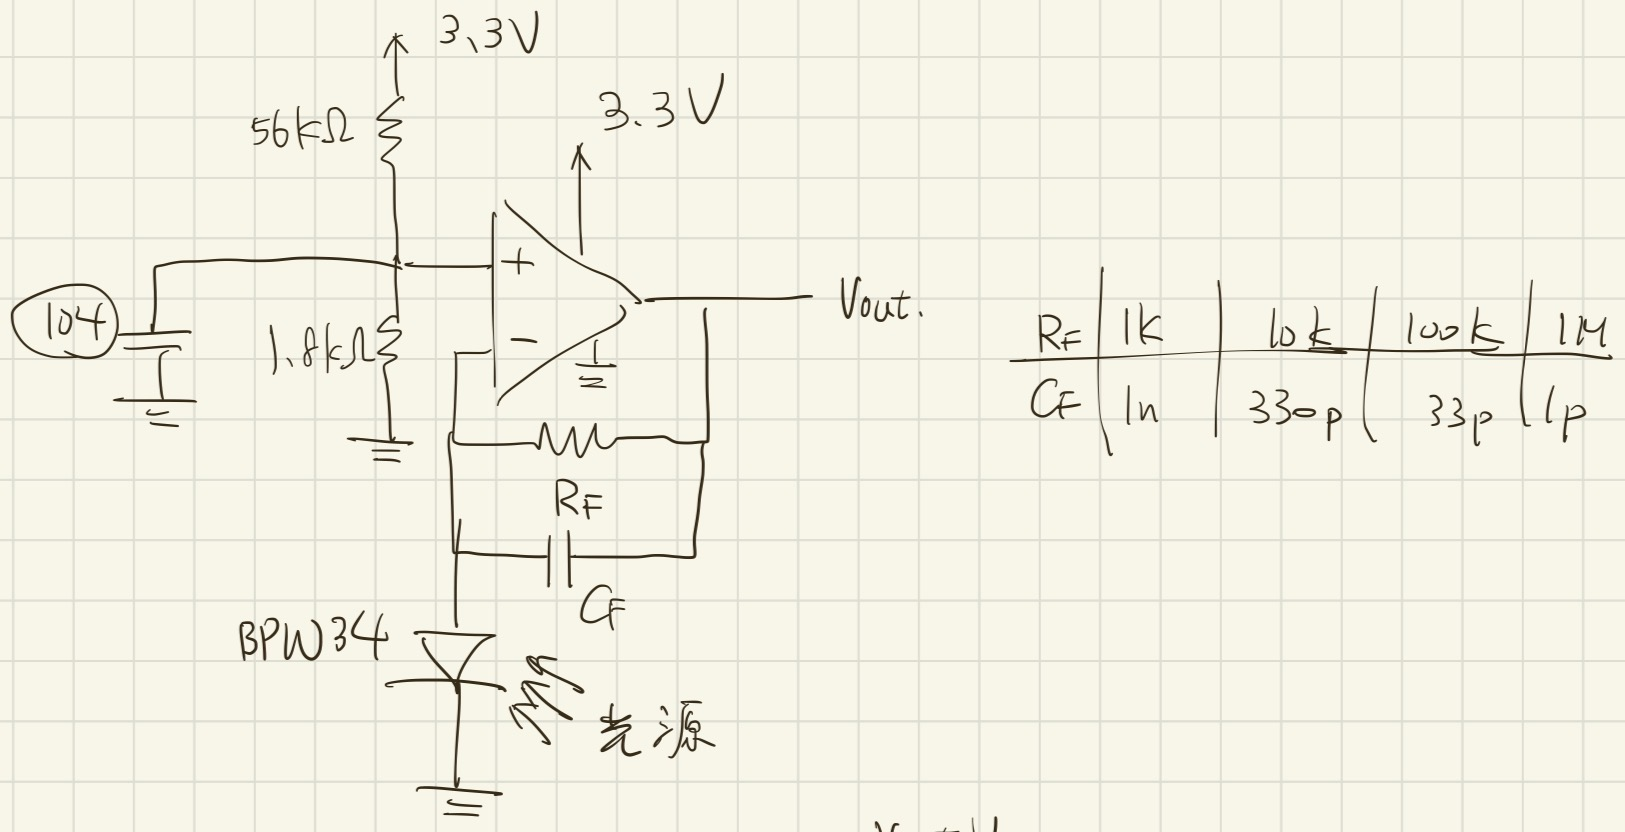
\includegraphics[width=0.9\linewidth]{2026-05-06/initial_schmatic.jpg}
  \caption{2026-05-06 麵包板 TIA 手繪圖。Op-amp 是 MCP6004,
           BPW34 接反相輸入端,非反相端透過 56 kΩ / 1.8 kΩ 分壓墊高到
           \(\sim \SI{0.103}{\volt}\)。回授 \(R_F\) 與 \(C_F\) 並聯,
           四檔增益配對見表~\ref{tab:0506-rfcf}。}
  \label{fig:0506-schematic}
\end{figure}

四檔 \(R_F / C_F\) 配對的思路是\textbf{讓 \(R_F C_F\) 乘積大致固定},
這樣每一檔的頻寬 \(f_{-3\text{dB}} = 1/(2\pi R_F C_F)\) 都落在差不多的範圍,
而不是讓低增益檔頻寬過高反而吃進更多雜訊。

\begin{table}[H]
  \centering
  \caption{四檔 \(R_F\)/\(C_F\) 配對與對應的小訊號頻寬。}
  \label{tab:0506-rfcf}
  \begin{tabular}{lllr}
    \toprule
    \(R_F\) & \(C_F\) & \(R_F C_F\) & 理論 \(f_{-3\text{dB}}\) \\
    \midrule
    1 kΩ   & 1 nF   & 1.0 μs & \(\sim\)159 kHz \\
    10 kΩ  & 330 pF & 3.3 μs & \(\sim\)48 kHz  \\
    100 kΩ & 33 pF  & 3.3 μs & \(\sim\)48 kHz  \\
    1 MΩ   & 1 pF   & 1.0 μs & \(\sim\)159 kHz \\
    \bottomrule
  \end{tabular}
\end{table}

50--150 kHz 的頻寬遠超過 20 kHz PWM 目標,所以四檔都能跑動態量測。
(註:\texttt{simulation/main.py} 的 DC 模擬為了簡化把 \(C_F\) 固定在 100 nF,
那是模擬端的近似,跟麵包板實際用的配對表不同。)

\subsection*{下午 3 點:功能驗證(手指遮光測試)}

電路接好後,先做最簡單的「手指遮光、看電表會不會動」測試,
確認光電轉換 + TIA 整條鏈路都活著。三用電表跨在 \(V_\text{OUT}\) 跟 GND 之間,
測試結果:

\begin{itemize}[leftmargin=2em,itemsep=0pt]
  \item 自然採光(無遮蔽,圖~\ref{fig:0506-light}):\(V_\text{OUT} = \SI{1.637}{\volt}\)
  \item 手指壓在 BPW34 感光面(圖~\ref{fig:0506-dark}):\(V_\text{OUT} = \SI{0.302}{\volt}\)
\end{itemize}

\(\Delta V \approx \SI{1.3}{\volt}\) 的明顯擺動,代表電路功能正確。

\begin{figure}[H]
  \centering
  \begin{minipage}{0.48\linewidth}
    \centering
    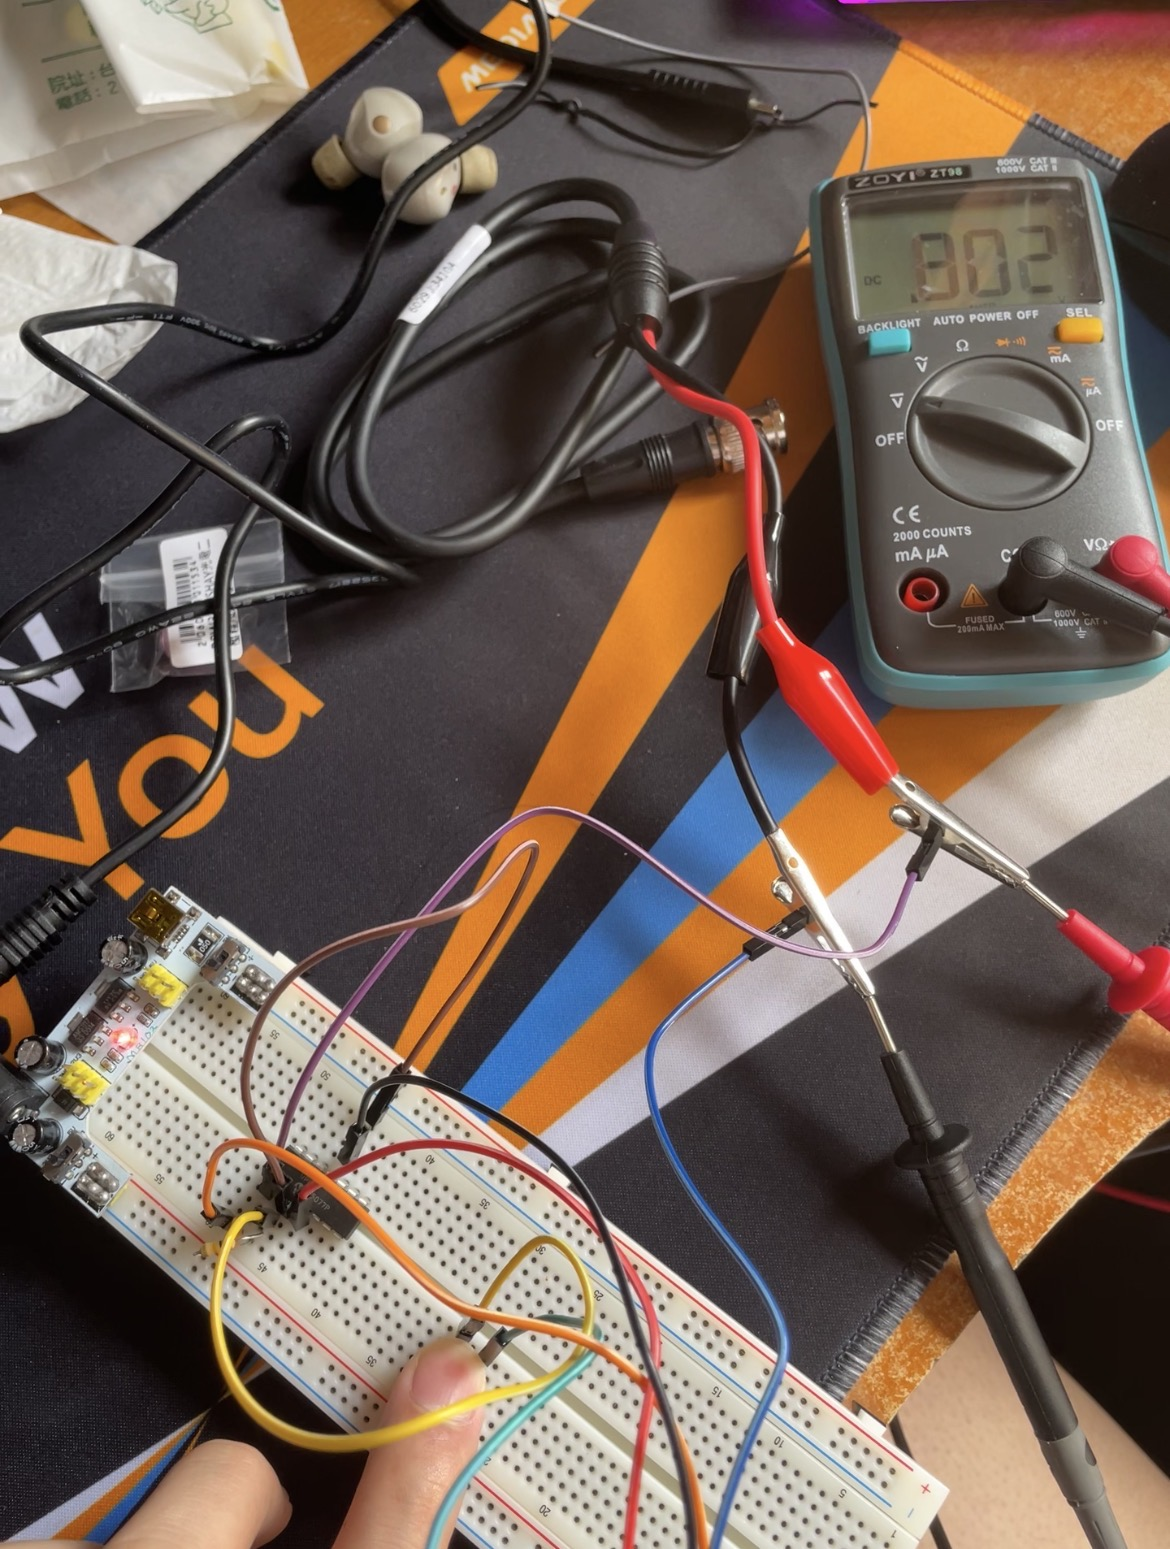
\includegraphics[width=\linewidth]{2026-05-06/BPW34_without_light.jpg}
    \caption{手指壓住 BPW34 受光面:\(V_\text{OUT} = \SI{0.302}{\volt}\)。
             無法完全壓到 \(V_\text{ref} \approx \SI{0.1}{\volt}\),
             差距來自漏光與 op-amp 的近 0 V 非線性。}
    \label{fig:0506-dark}
  \end{minipage}\hfill
  \begin{minipage}{0.48\linewidth}
    \centering
    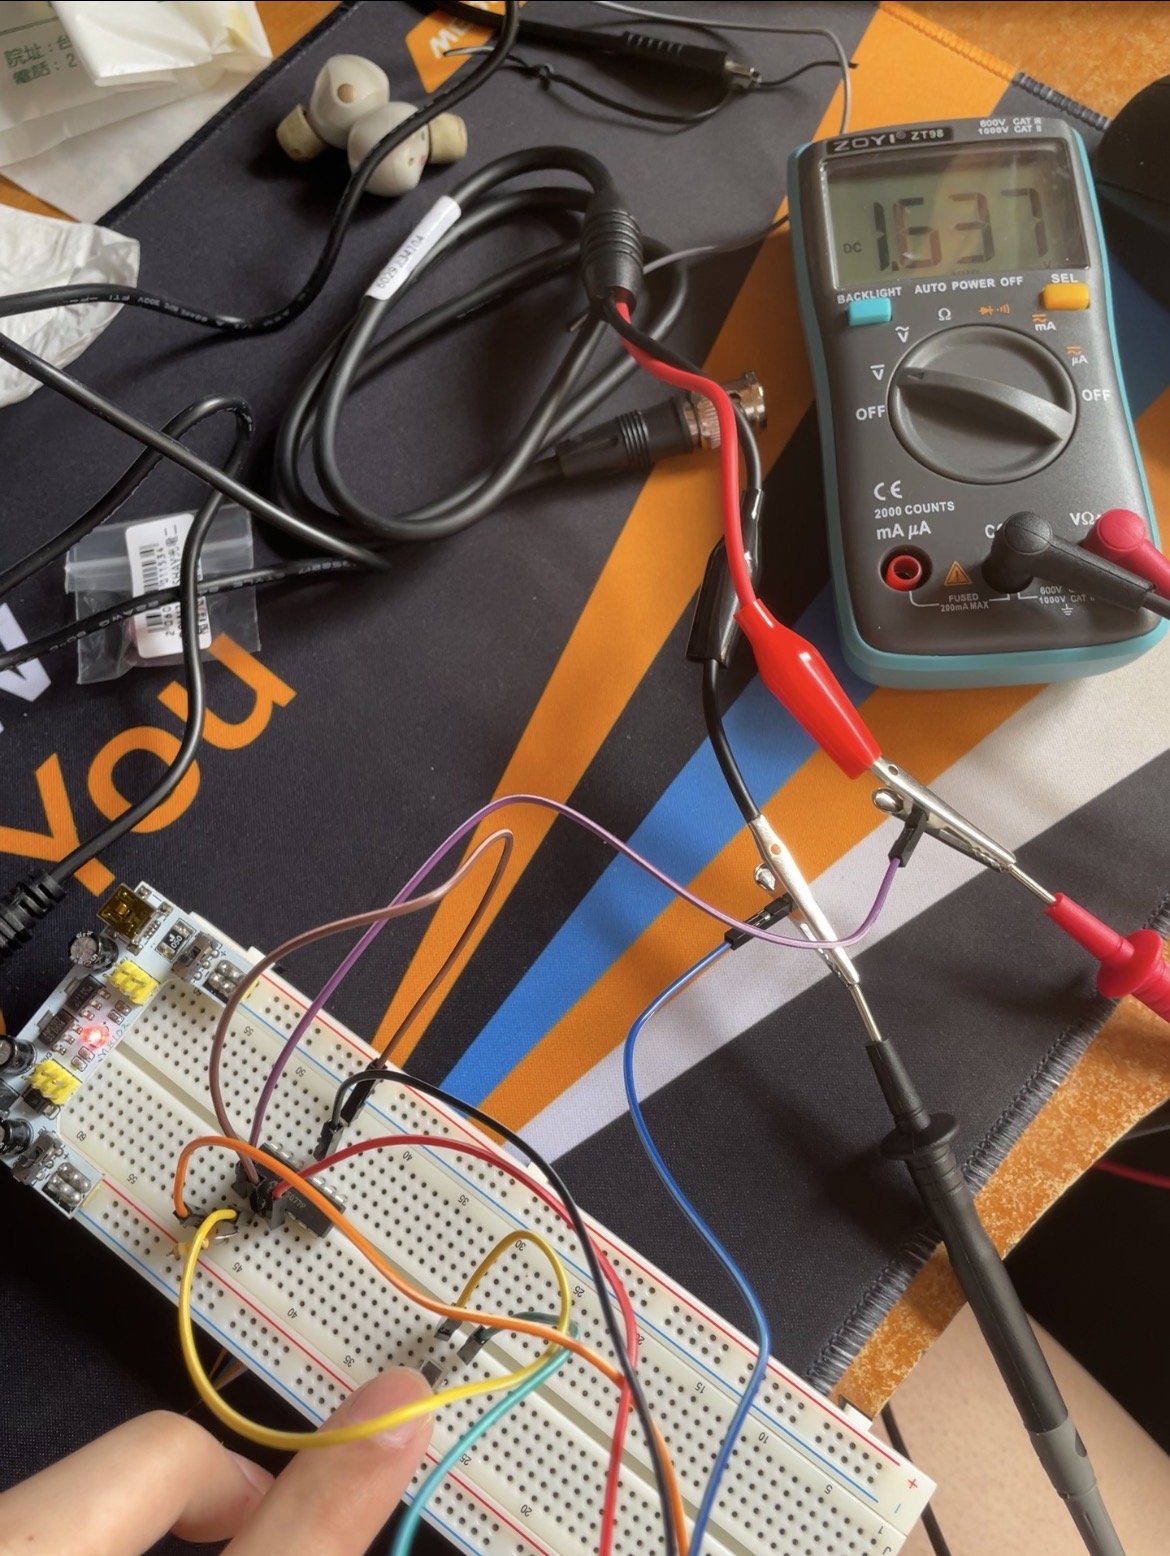
\includegraphics[width=\linewidth]{2026-05-06/BPW34_with_light.jpg}
    \caption{放開手指:\(V_\text{OUT} = \SI{1.637}{\volt}\)。
             正常室內採光下 TIA 輸出沒撞到上軌,動態範圍可用。}
    \label{fig:0506-light}
  \end{minipage}
\end{figure}

接著手動把 \(R_F\) 在四檔 \{1 kΩ, 10 kΩ, 100 kΩ, 1 MΩ\} 之間切換,
配對的 \(C_F\) 也跟著換,逐一在不同光照(全暗、白蓋、室內、手機手電筒)讀電表 ——
這就是下一節 4$\times$4 表的來源。

\subsection*{今天看到的痛點(下次採購清單)}

\begin{enumerate}[leftmargin=2em,itemsep=2pt]
  \item \textbf{杜邦線太亂}。麵包板上一旦同時掛 op-amp + 偏壓分壓 + 回授 + 量測點 + 三用電表線,
        20 cm 的杜邦線就會在板子上方繞成一坨。更糟的是,因為線太長 + BPW34 又長腳,
        \textbf{BPW34 沒辦法平貼到待測螢幕上} —— 一直被線拉住翹起來,
        感光面跟螢幕之間有明顯間隙,雜散光跑進去、訊號也不準。
        \textbf{下次採購:小跳線盒(預先剪好不同長度的硬跳線)} —— 線可以走平貼麵包板的水平路徑,
        感測元件就可以乖乖貼在螢幕上。
  \item \textbf{沒有四段波段開關}。每換一檔 \(R_F\) 都要拔線、換電阻、再插回去 ——
        4 個 \(R_F\) × 4 種光照 = 16 個讀數,每次都重接一次接線,容易插錯位、
        又會抖動電路擾動量測。
        \textbf{下次採購:1P4T 波段旋鈕開關} —— 跟 4/19 跟 Gemini 討論的方案接上,
        後續真的進外殼也用得到。
\end{enumerate}

\subsection*{量測程序與結果}

固定電路、轉動回授電阻 \(R_F\),分別在四種照度下用三用電表讀 \(V_\text{OUT}\)。原始紀錄留在
\texttt{simulation/data/exp\_260506.dat},整理表如下:

\begin{table}[H]
  \centering
  \caption{\(V_\text{OUT}\) (V) — 4 個 \(R_F\) × 4 種光照,2026-05-06 麵包板量測。}
  \label{tab:0506-bench}
  \begin{tabular}{lrrrr}
    \toprule
    \(R_F\) & Total Dark & White Cap & Room Light & Phone Flashlight \\
    \midrule
    1 MΩ    & 0.318  & 3.33   & 3.33   & 3.33  \\
    100 kΩ  & 0.024  & 0.523  & 1.342  & 3.33  \\
    10 kΩ   & 0.0031 & 0.0485 & 0.1352 & 2.40  \\
    1 kΩ    & 0.0058 & 0.0047 & 0.0113 & 0.214 \\
    \bottomrule
  \end{tabular}
\end{table}

每一個讀數 \(\SI{3.33}{\volt}\) 都是頂到電源軌的 clipping。

\subsection*{模擬 vs 量測比對}

PySpice 端跑 \texttt{simulation/main.py},四條 \(R_F\) 的 DC sweep \(V_\text{OUT}(I_\text{photo})\)
如圖~\ref{fig:0506-tia-sweep}。

\begin{figure}[H]
  \centering
  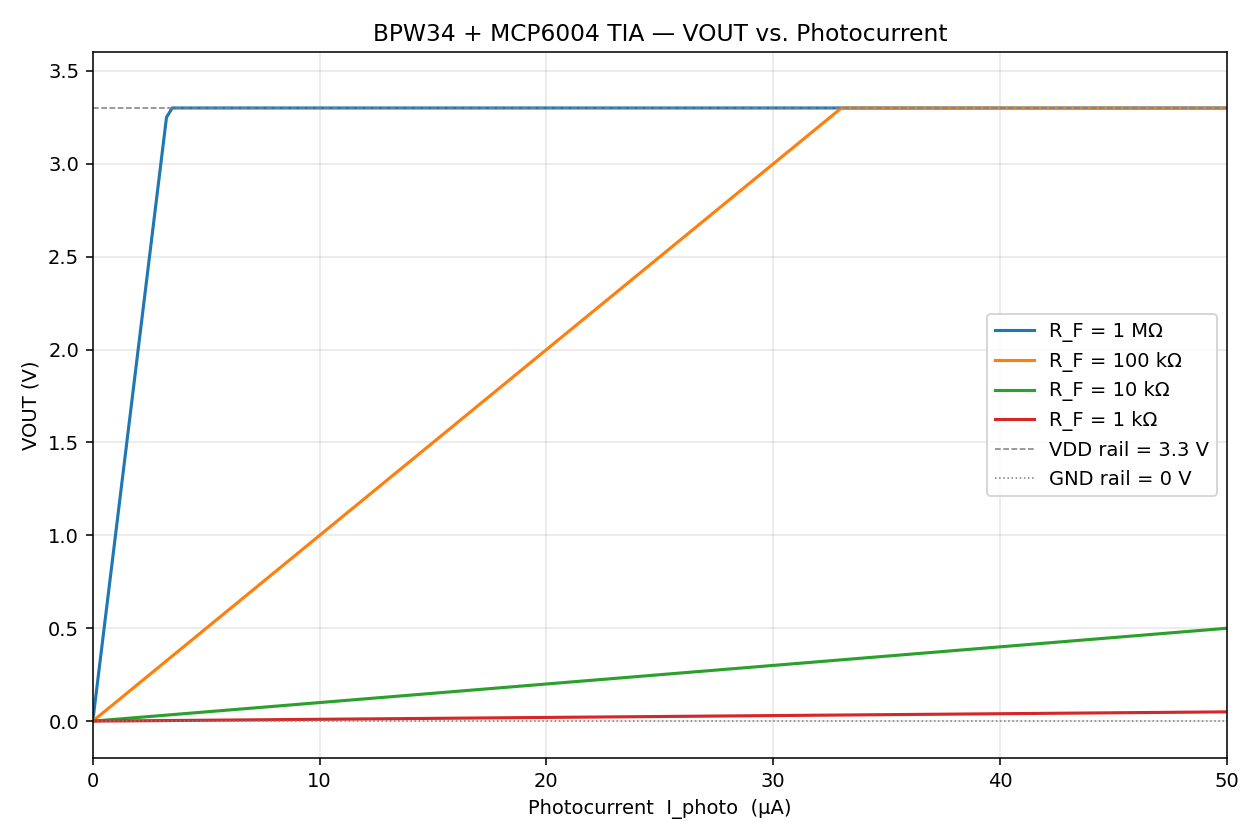
\includegraphics[width=0.85\linewidth]{2026-05-06/tia_sweep.png}
  \caption{PySpice DC sweep:四個 \(R_F\) 對應的 \(V_\text{OUT}\) vs \(I_\text{photo}\),
           上下軌位 0 V 與 \(V_{DD} = \SI{3.3}{\volt}\) 標出。 模擬完美呈現
           \(V_\text{OUT} = I_\text{photo} R_F\) 直到撞到上軌為止。}
  \label{fig:0506-tia-sweep}
\end{figure}

兩個對照點讓我們確認模擬與實際對得上:

\begin{itemize}[leftmargin=2em,itemsep=0pt]
  \item \textbf{線性增益}(Room Light 那一欄,100 kΩ 與 10 kΩ 都沒飽和):
        \(V_\text{OUT}\) 比值 \(1.342 / 0.1352 = 9.93\),對「理想 10×」誤差不到 1\%。
        反推光電流 \(I_\text{photo} = 13.42\) μA 與 \(13.52\) μA — 兩個獨立 \(R_F\)
        對同一物理量的估計差 0.7\%。
  \item \textbf{Clipping ceiling}:所有飽和讀值都落在 3.33 V,與模擬的 3.3 V 軌位
        差 30 mV(在三用電表標稱準度內)。每個 \(R_F\) 的 \(I_\text{clip} = V_{DD}/R_F\)
        都和飽和欄位一一對應 — \(R_F = 1\) MΩ 對應 \(I_\text{clip} = \SI{3.3}{\micro\ampere}\),
        一點點室內光就過頭;\(R_F = 1\) kΩ 對應 \(\SI{3.3}{\milli\ampere}\),手機手電筒
        近距離照都還在線性區。
\end{itemize}

\subsection*{非理想項解釋:為什麼 Total Dark 不是 0 V}

模擬下 \(I_\text{photo} = 0\) 給 \(V_\text{OUT} = 0\),但 bench 不是。把全黑欄位除以
\(R_F\) 反推 apparent input current:

\begin{itemize}[leftmargin=2em,itemsep=0pt]
  \item 三個高阻檔(1 MΩ / 100 kΩ / 10 kΩ)反推都是 \(\approx 250\)--\(320\) nA。
        \textbf{固定電流被 \(R_F\) 線性放大}的特徵,不是固定電壓 offset。
        最合理的來源是 \textbf{stray ambient light leakage} —— 房間光、電表 LED、
        手機螢幕的微弱漏光,任何一個都足以在 BPW34 的 \(\SI{7.5}{\square\milli\metre}\)
        感光窗上產生幾百 nA 的光電流(對應 μW 量級的光功率)。
  \item \(R_F = 1\) kΩ 時 \(V_\text{OUT}\) 升到 \(\SI{5.8}{\milli\volt}\) — 比理論 dark 還大,
        這時主導的是 \textbf{MCP6004 的輸入失調電壓 \(V_{os}\)}(spec 標 ±2 mV typical、
        ±4.5 mV max),不是光電流。在低 \(R_F\) 把光電流項壓下去後,
        op-amp 自身的 offset floor 才浮現。
\end{itemize}

把這兩個非理想項加進 PySpice 的網表很容易,但今天先停在「指認來源」這一步。

\subsection*{動態特性:用模擬挑 \(C_F\)}

固定 \(R_F = 100\) kΩ,把 \(C_F\) 掃 \{1 pF, 10 pF, 100 pF, 1 nF, 100 nF\},
跑 AC sweep(1 Hz–1 MHz)看 \(|Z(f)|\)、再跑 20 kHz 0–10 μA 方波 transient 看波形:

\begin{figure}[H]
  \centering
  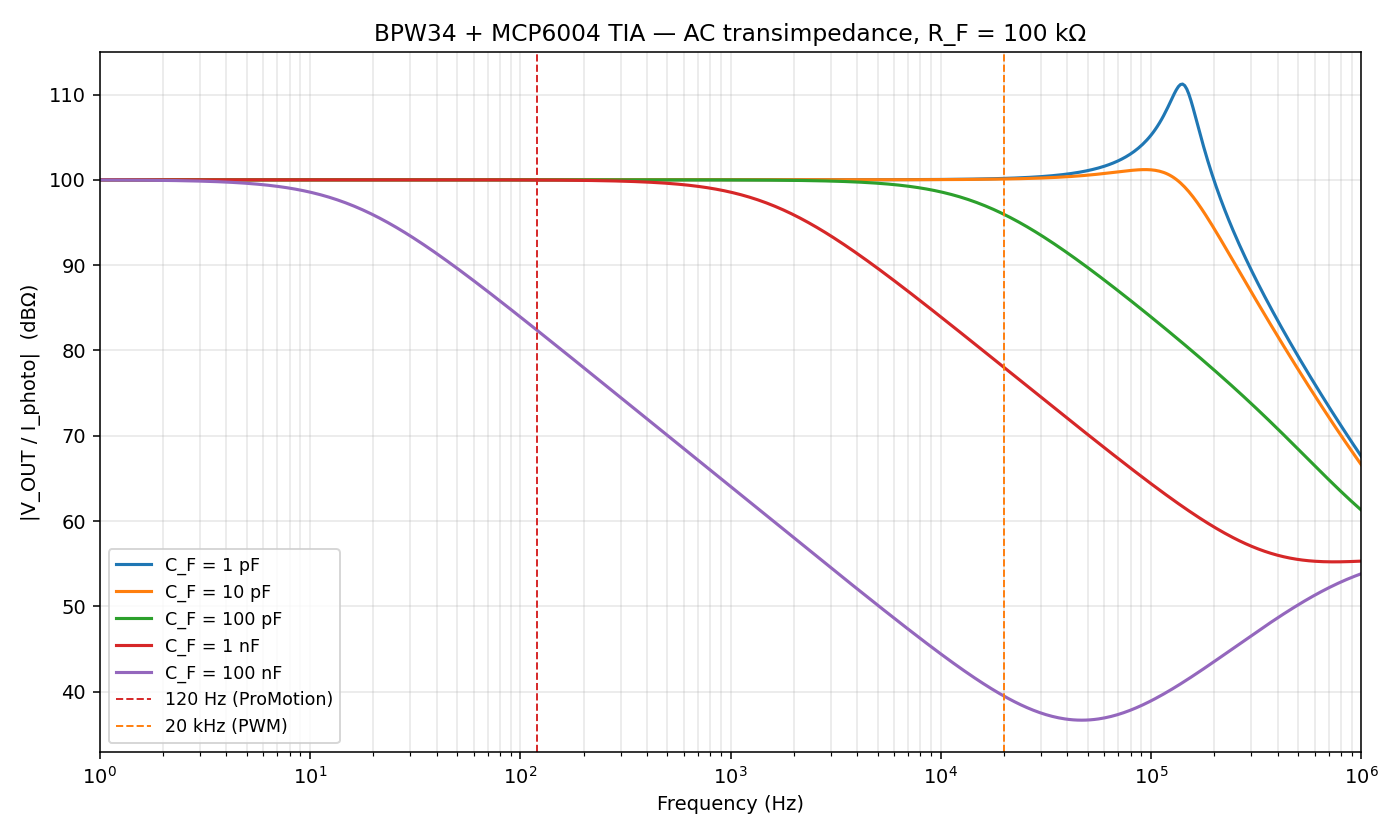
\includegraphics[width=0.85\linewidth]{2026-05-06/ac_bode.png}
  \caption{AC transimpedance \(|V_\text{OUT}/I_\text{photo}|\)。標出 120 Hz(ProMotion)
           與 20 kHz(PWM)兩個目標頻率。}
  \label{fig:0506-bode}
\end{figure}

\begin{figure}[H]
  \centering
  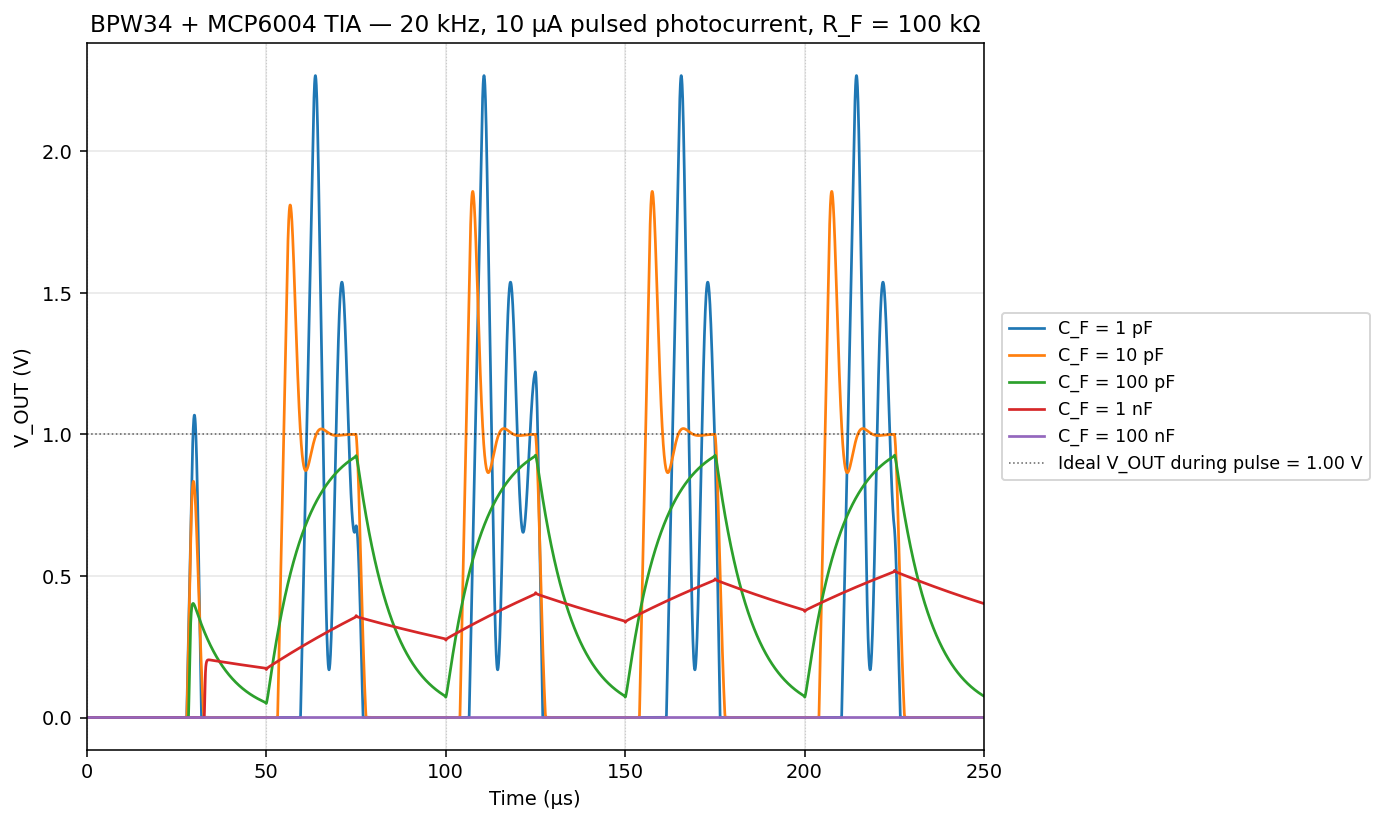
\includegraphics[width=0.85\linewidth]{2026-05-06/transient_pwm.png}
  \caption{20 kHz、10 μA 方波光電流的 transient 響應。理想 \(V_\text{OUT} = 1.0\) V。
           \(C_F = 1\) pF 嚴重 ringing、\(C_F \geq \SI{1}{\nano\farad}\) 變積分波形,
           中間的 10 pF 邊緣銳利又穩定。}
  \label{fig:0506-transient}
\end{figure}

從 Bode 跟 transient 一起看,各個 \(C_F\) 對兩個目標頻率的可用性:

\begin{table}[H]
  \centering
  \caption{\(R_F = 100\) kΩ 下,各補償電容 \(C_F\) 的可用性。}
  \label{tab:0506-cf}
  \begin{tabular}{lrcc}
    \toprule
    \(C_F\) & 模擬 \(f_{-3\text{dB}}\) & 120 Hz(ProMotion) & 20 kHz(PWM) \\
    \midrule
    1 pF   & 224 kHz           & 通過 & 通過(欠補償、有 ringing) \\
    \textbf{10 pF}  & \textbf{170 kHz} & \textbf{通過} & \textbf{通過(推薦)} \\
    100 pF & 16 kHz            & 通過 & 衰減 \(\sim\)\(-3\) dB,可用 \\
    1 nF   & 1.6 kHz           & 通過 & 砍掉 \\
    100 nF & 16 Hz             & 砍掉 & 砍掉 \\
    \bottomrule
  \end{tabular}
\end{table}

\textbf{推薦 \(C_F = 10\) pF}:既能保住 20 kHz PWM 邊緣,又比 1 pF 更穩、不會 ringing。
而今天 bench 上用的 \(C_F = \SI{100}{\nano\farad}\) 把 \(f_{-3\text{dB}}\) 壓到 16 Hz,
把 120 Hz 跟 20 kHz 兩個目標都吃掉了 —— 純 DC 量測沒事,但下次做動態量測前必須換掉。

\subsection*{今日心得}

\begin{itemize}[leftmargin=2em,itemsep=0pt]
  \item \textbf{TIA 理論驗證成功}:兩個獨立 \(R_F\) 對同一光電流的估計差 0.7\%、
        \(V_\text{OUT}\) 比值與 \(R_F\) 比值對到 1\% 內、clipping ceiling 與 \(V_{DD}\)
        對到 1\% 內 —— PySpice 跟麵包板真的對得起來,這份信心很關鍵。
  \item \textbf{Dark floor 不是 bug}:300 nA stray ambient + 5.8 mV \(V_{os}\) 都是
        datasheet 可查的真實效應,不是電路接錯。日後要進低光量測,得加遮光罩
        並且軟體做開機暗態校正。
  \item \textbf{\(C_F\) 是我 4/19 沒考慮到的東西}:4/19 只決定 \(R_F\) 用旋鈕切檔,
        以為 \(C_F\) 隨便挑。今天才知道 \(C_F = \SI{100}{\nano\farad}\)
        會把動態目標砍光,要改成 \(\sim \SI{10}{\pico\farad}\)。
  \item \textbf{ngspice + macromodel + PySpice 三層膠水}:libngspice SONAME、
        \texttt{set ngbehavior=ps} 時機、\texttt{Note:} 被當 fatal 這三個坑要記住,
        日後換機器重建環境一定會再撞。
  \item \textbf{下一步}:做動態量測前要先換 \(C_F\) 為 10 pF;同時開始想 Pico ADC
        的取樣率與 buffer 大小(2 kHz 對 ProMotion 1 Hz 需要長窗,10 kHz 對 PWM
        20 kHz 需要短窗,要兩套參數還是動態切換,還沒想清楚)。
\end{itemize}


\logentry{2026-05-07}{規劃購買烙鐵:從 TS101/TS21 比到 HS-02A}
% =====================================================================
%  2026-05-07 — 規劃購買烙鐵:從 TS101/TS21 比到 HS-02A
% =====================================================================

\subsection*{今日目標}

4/21 光華行裡列為「可以等(網購)」的烙鐵今天決定下單。請 Gemini 幫忙做選型,
重點是\textbf{精密 vs 通用熱容量}的取捨。

\subsection*{選型重點(濃縮)}

\begin{itemize}[leftmargin=2em,itemsep=0pt]
  \item \textbf{烙鐵頭系統決定一切}:
        \texttt{TS / T12}(中型、耗材便宜) vs \texttt{C210}(極精密、秒熱)
        vs \texttt{C245}(精密又有熱容、能扛粗線/BNC) —— 是兩個極端與一個中間值。
  \item \textbf{功率不等於溫度}:功率代表回溫速度;PD 3.1 / 100 W 是目前主流。
  \item \textbf{供電}:USB-C PD 是現代趨勢,可以用筆電充電頭、行動電源供電,
        實驗室桌面不用再多拉一條 AC。
  \item \textbf{安全}:自動休眠 + ESD safe + 接地 三個基本。
\end{itemize}

\subsection*{Miniware TS101 vs TS21}

\begin{itemize}[leftmargin=2em,itemsep=0pt]
  \item \textbf{TS101} —— TS 系列(類 T12)頭,DC 5525 + USB-C 雙接口,
        65 W (DC) / 90 W (PD),\textbf{萬用工具箱型}。
  \item \textbf{TS21} —— C210 整合芯,僅 USB-C、100 W PD 3.1、3--5 秒熔錫,
        全金屬機身、附補光燈,\textbf{精密手術刀型}。
  \item 結論:TS21 的 C210 頭對螢幕貼螢幕的微焊接很順手,
        但要焊 BNC / 粗導線時熱容會吃力 —— 對 flico 這種要焊 SFH 2440 + Pico 排針
        + 偶爾接線材的混合場景,光 C210 太極端。
\end{itemize}

\subsection*{擴大比較範圍(不限 Miniware)}

Gemini 又列了四個競品系統:

\begin{itemize}[leftmargin=2em,itemsep=0pt]
  \item \textbf{Fnirsi HS-02B}(C210)—— TS21 的直接對手,附金屬保護蓋,
        用完不用等冷卻直接收。
  \item \textbf{Fnirsi HS-02A}(C245)—— \emph{同系列但用 C245 較大發熱芯};
        熱容大、能扛粗線,也保留精密能力。
  \item \textbf{Alientek T100 / T90B}(C210 / C245)—— 韌體穩定、顯示資訊詳盡。
  \item \textbf{PTS200 V2} —— ESP32 控制,TS / T12 通殺,開源韌體可玩。
  \item \textbf{Pinecil V2}(TS / T12)—— 開源 IronOS,CP 值最高,
        但機身輕到容易被線材帶走、頭至手握距離長對微焊接不利、
        外殼塑膠感較重。
\end{itemize}

Gemini 對我的建議是「物理系學生混合場景應選 C245 系統(HS-02A 或 S99),
C210 在焊 BNC 接頭時會吃力」 —— 這跟我的需求對上。

\subsection*{購買決定 \& 物流}

\begin{itemize}[leftmargin=2em,itemsep=0pt]
  \item 機型:\textbf{Fnirsi HS-02A}(C245 發熱芯,PD 3.1, 最高 100 W,金屬保護蓋)
  \item 價格:\textbf{TWD 968}
  \item 下訂單:\textbf{2026-05-07 (三) 23:33}
  \item 到貨/取件:\textbf{2026-05-11 (日) 13:25}
\end{itemize}

\subsection*{今日心得}

\begin{itemize}[leftmargin=2em,itemsep=0pt]
  \item 烙鐵這種「一輩子買幾次」的工具值得花一晚上做功課;
        選錯系統(尤其是 C210 太精密扛不住粗線、或 T12 太大扛不住 SMD)
        會卡接下來整個專案的焊接環節。
  \item C245 是「精密 + 熱容」的中間值,符合 flico 之後要做的事:
        SFH 2440 SMD 上轉接板、Pico 排針、BNC 杜邦線、PCB 跳線都會碰到。
  \item Pinecil V2 雖然 CP 值漂亮但「頭至手握距離長」對 SMD 不利,排除。
  \item 取件當天再寫一篇開箱 / 第一次焊接的日誌。
\end{itemize}


\logentry{2026-05-08}{Pico + MicroPython 上線:打通完整訊號鏈}
% =====================================================================
%  2026-05-08 — Pico + MicroPython 上線,打通完整訊號鏈
% =====================================================================

\subsection*{今日目標}

\begin{itemize}[leftmargin=2em,itemsep=0pt]
  \item 用 5/6 驗證過的 \textbf{BPW34 + MCP6004 TIA} 餵 \textbf{Raspberry Pi Pico} 做 ADC 擷取,
        驗證對 \textbf{20 kHz PWM} 與 \textbf{120 Hz 螢幕閃爍} 的量測能力。
  \item Pico 端\textbf{用 MicroPython 寫原型}:edit/save/run loop 比 C++ Pico SDK 的
        CMake/編譯/燒寫快太多,先求功能跑通再說。
        (日後若效能撐不住再轉 C++,但今天還早。)
  \item 三段全打通:VS Code MicroPython 環境 → Pico ADC 採樣 → USB-CDC 串到 PC 端 \texttt{pyserial}。
        (本來打算順手把 I\textsuperscript{2}C OLED 也接上,但 OLED 還沒到貨,留 5/11 採購回來再做。)
\end{itemize}

\subsection*{階段一:MicroPython + VS Code 環境驗證}

第一個提示詞(精簡版,完整對話留待之後補檔):

\begin{quote}\small
請提供一個在 Raspberry Pi Pico 上運行的 MicroPython 基礎 LED 閃爍(Blink)程式碼,
並說明如何在 VS Code 環境下透過 MicroPython 擴充功能將程式燒錄與執行。
\end{quote}

\begin{itemize}[leftmargin=2em,itemsep=0pt]
  \item 結果:VS Code 的 MicroPython extension 設妥,Pico 燒入 MicroPython UF2 韌體後
        被識別為 serial device;\texttt{blink.py} 上板成功亮滅,
        \emph{edit \(\to\) save \(\to\) run} 流程暢通。
  \item 對應檔:\texttt{firmware/led-light-test-python-version/blink.py}(14 行,只開 \texttt{Pin("LED")} toggle)。
        子資料夾尾巴的 \texttt{-python-version} 是為了之後若回去寫 C++/Pico-SDK 對照版本,
        可以平行放 \texttt{led-light-test-cpp-version/} 不會打架。
  \item \textbf{意義}:這是 flico 從「類比量電壓」進到「數位 ADC 擷取」的環境基石;
        沒有這一步,後面所有 Python 程式都跑不起來。
\end{itemize}

\subsection*{階段二:Pico ADC 採樣與 USB-CDC 串流}

第二個提示詞:

\begin{quote}\small
我需要使用 Pico 的 ADC 讀取光敏訊號,並透過 USB-CDC 即時把採樣值丟回電腦。
請提供 \texttt{main.py} 的主程式架構,確保能穩定採樣與輸出。
\end{quote}

\begin{itemize}[leftmargin=2em,itemsep=0pt]
  \item ADC 接腳:\texttt{ADC0 = GP26} 直接吃 MCP6004 TIA 的 \(V_\text{OUT}\)。
  \item \texttt{main.py} 在 idle loop 裡:讀 \texttt{adc.read\_u16()}、換算成電壓、
        透過 USB-CDC(\texttt{sys.stdout})往 PC 印一行純文字。
        \textbf{今天沒有顯示器,純流式輸出。}
  \item 對應檔:\texttt{firmware/python-version/main.py}。
        資料夾名取 \texttt{python-version} 是為了之後可平行放 \texttt{cpp-version/} 對照,
        本日是 MicroPython 路線。
        (現存版本是日後幾天迭代後加上 binary streaming、74HC4051 gear 切換、GAP marker、
        以及 SSD1306 OLED 顯示等的成熟版;
        5/8 當天的初版只有 ADC + 印一行字到 stdout、\textbf{沒有 OLED} ——
        OLED 是 5/11 買到自己的 0.91" 螢幕、寫 \texttt{ssd1306.py} 之後才接上去的。)
\end{itemize}

\subsection*{階段三:PC 端 pyserial 接收}

第三個提示詞:

\begin{quote}\small
請寫一個在電腦(PC)端運行的 Python 腳本,透過 \texttt{pyserial} 讀取連接在 USB 埠的
Pico 傳送出來的 ADC 採樣數據,並將資料即時列印或儲存,以便分析 TIA 電路擷取到的閃爍(Flicker)訊號。
\end{quote}

\begin{itemize}[leftmargin=2em,itemsep=0pt]
  \item 結果:\texttt{read\_data.py} 開 \texttt{/dev/cu.usbmodemXXX}(macOS),
        阻塞讀 USB-CDC 行,印到 console。簡單粗暴但訊號鏈通了。
  \item 對應檔:\texttt{host/read\_data.py}。
        (現存版本同樣已長成完整 PyQtGraph dashboard:多 rate view table、smart auto-tracking、
        CSV 匯出 ——這是後續幾天演化的結果,5/8 當天只有一個 \texttt{while True: print(ser.readline())}。)
  \item \textbf{放在 host/ 而非 firmware/} 的理由:這支跑在電腦上,不在 Pico 上 —— flico 把 PC 端工具
        統一放 \texttt{host/}。
\end{itemize}

\subsection*{動態驗證:experiment\_result.MOV}

實機錄影留底:\texttt{figures/2026-05-08/experiment\_result.MOV}(21 MB)。
畫面內容:

\begin{itemize}[leftmargin=2em,itemsep=0pt]
  \item 手指接近 / 遠離 BPW34 感光面
  \item PC 端 console 同步印出 ADC 數值的擺動
\end{itemize}

\textbf{整條訊號鏈「BPW34 \(\to\) MCP6004 TIA \(\to\) Pico ADC \(\to\) USB-CDC \(\to\) PC pyserial」確認活著。}

\subsection*{今天另一條線:下載 KiCad,第一次嘗試畫 PCB}

訊號鏈跑通之後天還沒黑,順手做了第二件事:\textbf{下載 KiCad}(8.0)、
開了一個叫 \texttt{pico\_flicker\_shield} 的專案、試著把 5/6 麵包板上那塊 TIA
搬到正式 schematic 上。\textbf{不是要這次就送 JLCPCB,只是想趁印象還新的時候
把那塊電路落地成「Pico shield」形式存檔}—— 之後麵包板拆掉,還有紙本可以回顧。

\begin{itemize}[leftmargin=2em,itemsep=0pt]
  \item \textbf{流程選 KiCad 原生 GUI workflow}:Schematic Editor 拉線、選 symbol、
        annotate、選 footprint。完全沒用 SKiDL(那是 5/18 才會切換的程式化路線)。
  \item \textbf{當天的 schematic 主體}:Pico header(母排針 \(2 \times 20\)) +
        BPW34 + MCP6002(雙 op-amp,SOIC-8 SMD) + 4 顆回授電阻
        (1\,k / 10\,k / 100\,k / 1\,M) + 4 顆配對 \(C_f\) + 74HC4051 mux(DIP-16)
        作為換檔元件。直接照 5/3 提案書那張電路圖畫,沒有對元件規格做升級。
  \item \textbf{今天只完成 schematic 階段,PCB layout 沒動}—— ratsnest 還沒拉、
        footprint 還沒擺。今天的目標是「\textbf{學會用 KiCad}」,不是「\textbf{做出來投產的 PCB}」。
  \item 對應檔:\texttt{hardware/first-version/pico\_flicker\_shield.kicad\_sch}
        (今天 17:08 存檔)。PCB 那個 \texttt{.kicad\_pcb} 是空白的、後續日子才會慢慢填。
\end{itemize}

\textbf{重要:這個 \texttt{first-version} 後來會被放棄。} 原因要等 5/18 才會浮上來:
那天會發現 GUI workflow 在反覆改規格時 diff 完全沒辦法 review、改一次要拖一次 GUI,
改用 SKiDL 程式化從零重寫,新的版本叫 \texttt{PD\_detector\_pro},歸檔在
\texttt{hardware/second-version/}。但 \texttt{pico\_flicker\_shield} 留著當這條設計史
的第一筆,所以 \texttt{hardware/first-version/} 不刪。

\subsection*{今日心得}

\begin{itemize}[leftmargin=2em,itemsep=0pt]
  \item \textbf{從類比走進數位的橋樑搭起來了} —— 5/6 還停在三用電表手動讀電壓,今天就有完整端到端的程式化擷取。
  \item \textbf{MicroPython 對原型開發是巨大的加速}。改一行存檔就跑,
        不用 C++ Pico SDK 那套 CMake/編譯/燒寫的循環。
        功能跑通之後若效能不夠再改 C++,但今天還早。
  \item \textbf{切「韌體」vs「PC 端」的界線在 commit 時就釐清}:\texttt{main.py} 放
        \texttt{firmware/python-version/} 因為跑在 Pico 上;\texttt{read\_data.py} 放 \texttt{host/} 因為跑在電腦上。
        兩邊以 USB-CDC ASCII / binary 協定為唯一耦合點。
  \item \textbf{下一步}:
        \begin{enumerate}[leftmargin=2em,itemsep=0pt]
          \item 把 0.91" SSD1306 OLED 接上去,讓 Pico 自己也能秀瞬間電壓 —— 等 5/11 採購回來再做。
          \item PC 端把 console print 換成 numpy FFT + 即時繪圖(後來才知道 matplotlib 在 macOS 全螢幕重繪會閃,
                會走到 PyQtGraph)。
          \item Pico 端 ADC 取樣率得做到 \(\geq 10\) kHz 才能可靠抓 20 kHz PWM 的諧波;
                目前是輪詢式單樣本,要改成 DMA / timer-driven。
          \item KiCad schematic 起手了,接下來繼續把 footprint 配齊、ratsnest 拉一拉、
                把 PCB layout 慢慢打磨。預計花 1\(\sim\)2 週的零碎時間,
                目標還只是「看自己畫得出來嗎」,不是「投產」。
        \end{enumerate}
\end{itemize}


\logentry{2026-05-11}{第二次去光華:用 MUX 把波段開關吃掉的關鍵 insight}
% =====================================================================
%  2026-05-11 — 第二次去光華:用 MUX 把波段開關吃掉的關鍵 insight
% =====================================================================

\subsection*{今日目標}

\begin{itemize}[leftmargin=2em,itemsep=0pt]
  \item 回光華補 4/21 漏買的東西 \texttt{+} 解掉 5/6 麵包板實驗暴露出來的兩個痛點。
  \item 順路取 5/7 下單的 \textbf{Fnirsi HS-02A} 烙鐵(取件 13:25)。
  \item 把 5/3 那張「四檔旋鈕」的設計圖再升級一階:用 MCU 控制的類比 mux 取代純機械的波段開關。
\end{itemize}

\subsection*{關鍵 insight:用 ADC 動態範圍當「自動切檔」訊號}

5/6 量測復盤的時候發現一件事:Pico ADC 雖然名義上吃 0--3.3 V,但兩端各有一塊 dead zone:

\begin{itemize}[leftmargin=2em,itemsep=0pt]
  \item 下限:5/6 在 TIA 的 \(+\) 端故意墊了 \(V_\text{ref} \approx \SI{0.1}{\volt}\),
        所以 \(V_\text{OUT}\) 永遠 \(\gtrsim 0.1\) V;再加 op-amp 接近 0 V 的非線性,
        實際可用下限 \(\approx \SI{0.3}{\volt}\)。
  \item 上限:rail-to-rail 雖然能到 3.3 V,但接近上軌也有非線性 + clipping;
        實際可用上限 \(\approx \SI{3.0}{\volt}\)。
\end{itemize}

也就是「線性可用區」其實只有 \(\sim \SI{0.3}{\volt}\)--\(\SI{3.0}{\volt}\) 這一段。
原本以為兩端 dead zone 是浪費,但反過來看:它們其實是\textbf{現成的「該換檔了」訊號}。

\begin{itemize}[leftmargin=2em,itemsep=0pt]
  \item \(V_\text{OUT} \to \SI{3.0}{\volt}\) \(\Rightarrow\) 飽和了 \(\Rightarrow\) 該往\textbf{低增益}檔切。
  \item \(V_\text{OUT} \to \SI{0.3}{\volt}\) \(\Rightarrow\) 底噪了 \(\Rightarrow\) 該往\textbf{高增益}檔切。
  \item \(V_\text{OUT}\) 落在 \(0.3\)--\(3.0\) 中間 \(\Rightarrow\) 維持當前檔。
\end{itemize}

只要把 Pico 程式裡塞個 hysteresis-based 自動換檔狀態機,就能讓 flico
\textbf{不用人手動轉旋鈕}就在四檔之間無縫滑動。這是「智慧 flico」的第一個雛形。

\subsection*{硬體實作:74HC4051 取代機械式波段開關}

要讓 Pico GPIO 能切換 \(R_F\) 路徑,需要一顆\textbf{類比多工器 (analog multiplexer)}:

\begin{itemize}[leftmargin=2em,itemsep=0pt]
  \item 元件:\textbf{74HC4051}(8 通道單刀類比 mux,但這裡只用 4 通道對應四檔)。
  \item 接法:把 \texttt{COM} 接到 op-amp 的反相輸入,\texttt{Y0--Y3} 各接一顆 \(R_F\)
        (1 k / 10 k / 100 k / 1 M),另一端統一接 \(V_\text{OUT}\)。
        Pico GPIO 控 \texttt{S0/S1}(\texttt{S2} 拉地)做四選一。
  \item 4/19 跟 Gemini 討論時就提過 TMUX1104 這條路,當時覺得太進階,
        今天決定直接走 mux。74HC4051 在光華有貨、便宜、DIP 封裝可插麵包板,門檻最低。
  \item 雖然採購了一顆\textbf{傳統 1P4T 波段開關備援}(50 元),先當 fallback;
        若 mux 自動換檔搞不出來,還可以手動切。
\end{itemize}

\subsection*{順手解掉 5/6 留下的兩個痛點}

\begin{enumerate}[leftmargin=2em,itemsep=2pt]
  \item \textbf{杜邦線太亂、BPW34 翹起來貼不到螢幕} \(\to\) 買了 \textbf{140 根預剪硬跳線盒}。
        硬跳線可以走平貼麵包板的水平路徑,BPW34 就能乖乖貼螢幕了。
  \item \textbf{每換一檔 \(R_F\) 都要拔線} \(\to\) 上面的 74HC4051 mux 直接幹掉這件事,
        而且還順便升級成「MCU 自動切」(原本只是想要旋鈕)。
\end{enumerate}

\subsection*{今天另一條線:第一次接 OLED 用 I\textsuperscript{2}C 跑 SSD1306}

5/8 那天本來打算順手把 OLED 也接上,但當時沒貨;今天買到自己的 \textbf{0.91" SSD1306 OLED} 就把這條線補完,
flico 第一次有了「Pico 自己也會講話的螢幕」。

\begin{itemize}[leftmargin=2em,itemsep=0pt]
  \item \textbf{接腳}:I\textsuperscript{2}C0,\texttt{SDA=GP4 / SCL=GP5};
        OLED 預設 7-bit 地址 \texttt{0x3C}、解析度 \(128 \times 32\)。
  \item \textbf{驅動}:從 0 寫了 \texttt{ssd1306.py},繼承 MicroPython 內建的 \texttt{framebuf.FrameBuffer};
        提供兩個 class:
        \begin{itemize}[leftmargin=2em,itemsep=0pt]
          \item \texttt{SSD1306} —— 底層 \texttt{init\_display()} 寫 OLED 控制字
                (set MUX ratio / segment remap / charge pump 等十幾個命令),
                以及 \texttt{show()} 把 framebuf 推進顯示記憶體。
          \item \texttt{SSD1306\_I2C(SSD1306)} —— I\textsuperscript{2}C 包裝層,
                \texttt{write\_cmd} 走控制 byte \texttt{0x80}、
                \texttt{write\_data} 用 \texttt{writevto} 一次推 framebuf 整塊。
        \end{itemize}
  \item \textbf{整合到 main.py}:
        \texttt{oled.fill(0)} \(\to\) \texttt{oled.text("V=...", 0, 0)} \(\to\) \texttt{oled.show()}
        三步把瞬間電壓秀到螢幕。同樣的 ADC 讀取迴圈,5/8 還只是 print 到 console,
        今天\textbf{連電腦都不用接也能看讀數}。
  \item 對應檔:\texttt{firmware/python-version/ssd1306.py}(99 行,大半是 SSD1306 啟動序列那一段)。
\end{itemize}

把這條線打通的瞬間,5/3 提案書畫的「裝置正面」配置(感光窗 + 4 位 7 段顯示器 + 旋鈕 + 模式開關)
開始跟現實對得起來 —— 雖然今天用的是 OLED 不是 7 段,但 \textbf{flico 已經是一台「站著也能用」的儀器了},
不再是麵包板加一條杜邦線到三用電表那種「躺著實驗」階段。

\subsection*{購買清單與收據}

12:51 結帳於\textbf{今華電子}(同 4/21 那家),刷掉 \(\textbf{TWD 735}\) 現金、找回 65 元
(付 800)。收據如圖~\ref{fig:0511-receipt}。

\begin{figure}[H]
  \centering
  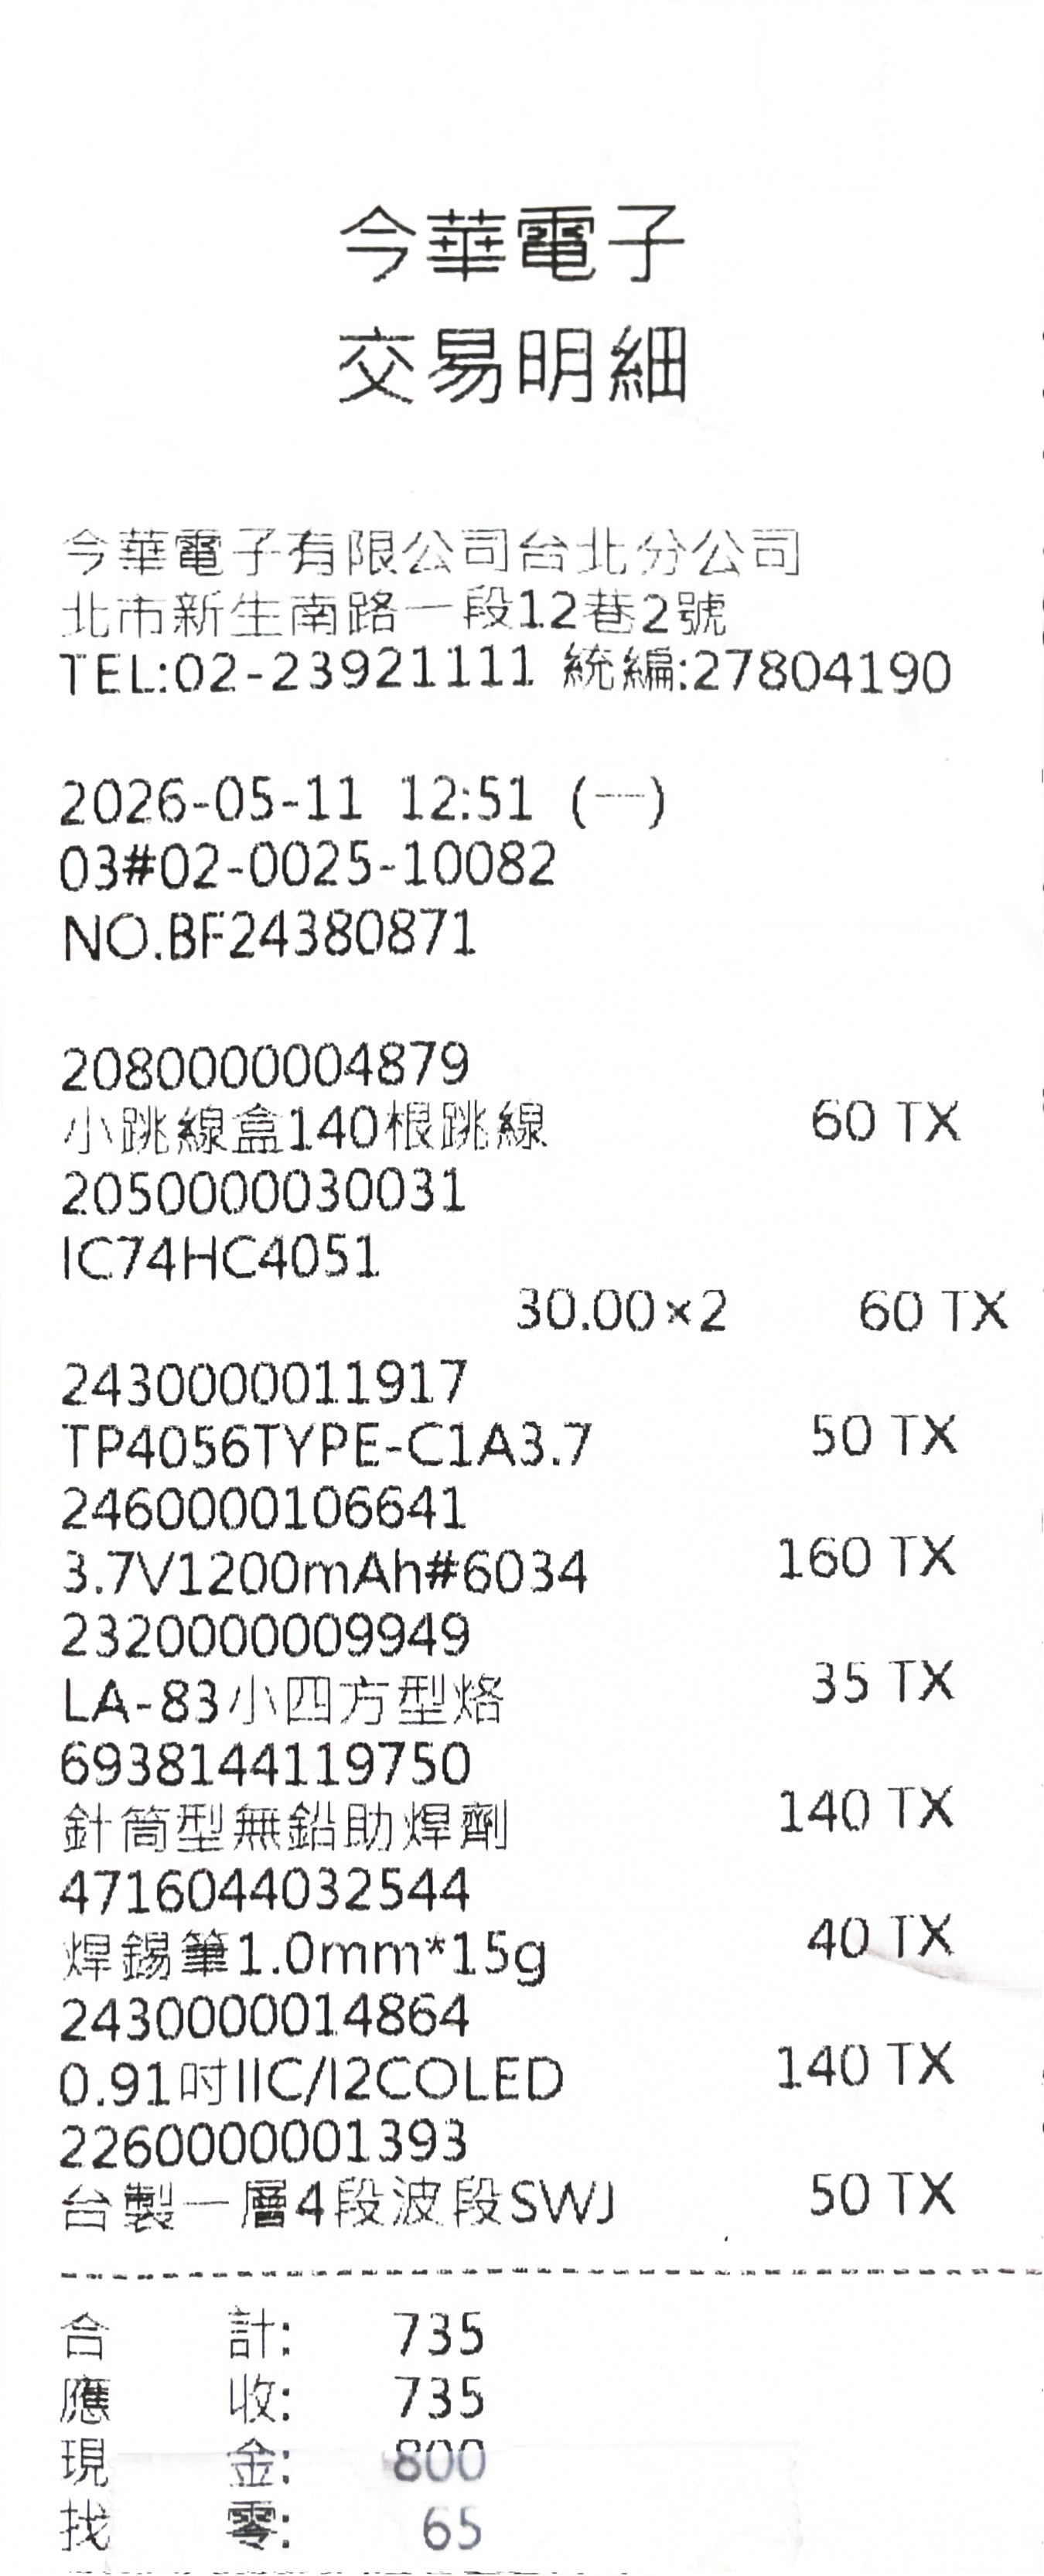
\includegraphics[width=0.55\linewidth]{2026-05-11/今華電子交易明細0511.jpg}
  \caption{今華電子 2026-05-11 12:51 第二次交易明細,合計 TWD 735。}
  \label{fig:0511-receipt}
\end{figure}

\begin{table}[H]
  \centering
  \caption{5/11 今華電子採購明細。}
  \label{tab:0511-bom}
  \begin{tabular}{llrr}
    \toprule
    類別 & 品項 & 數量 & 小計 (TWD) \\
    \midrule
    接線     & 小跳線盒 140 根預剪跳線              & 1 & 60  \\
    增益切換 & 74HC4051 8 通道類比 MUX(DIP-16)     & 2 & 60  \\
    增益切換 & 台製 1 層 4 段波段開關(備援)         & 1 & 50  \\
    電源     & TP4056 Type-C 1A 鋰電池充電板         & 1 & 50  \\
    電源     & 3.7 V / 1200 mAh LiPo 電池(\#6034)    & 1 & 160 \\
    顯示     & 0.91" I\textsuperscript{2}C SSD1306 OLED & 1 & 140 \\
    焊接     & LA-83 小四方形烙鐵架(海綿底座)        & 1 & 35  \\
    焊接     & 針筒型無鉛助焊劑(松香膏)              & 1 & 140 \\
    焊接     & 焊錫筆 1.0 mm \texttimes{} 15 g       & 1 & 40  \\
    \midrule
    \multicolumn{3}{r}{\textbf{合計(付現)}} & \textbf{735} \\
    \multicolumn{3}{r}{\textbf{付 800,找 65}} & \\
    \bottomrule
  \end{tabular}
\end{table}

幾個現場決定的細節:

\begin{itemize}[leftmargin=2em,itemsep=0pt]
  \item \textbf{74HC4051 ×2}:第二顆是備援,寒流發抖手抖燒一顆便宜很多。
  \item \textbf{TP4056 加上 LiPo 一起買}:5/3 提案書時候就決定電源走「3.7 V LiPo \(\to\) LDO \(\to\) 3.3 V」,
        今天把上游一次備齊;LDO 之前光華沒貨,留作下次。
  \item \textbf{0.91" OLED}:5/8 本來想接 OLED 但根本沒貨,今天先把感測器買回家,
        當天稍晚才正式接上去跑(詳上節「今天另一條線」)。
  \item \textbf{LA-83 烙鐵架 + 助焊劑 + 焊錫}:都是 5/7 下單烙鐵的配套耗材,
        準備今天 13:25 取件回家就直接焊。
\end{itemize}

回家拆袋順手拍了 LiPo 電池實物,做個檔案備存(圖~\ref{fig:0511-lipo});
注意黃色絕緣膠帶下面就是保護板,使用前要確認 TP4056 模組的 B\(+\)/B\(-\) 不能跟電池正負極接反。

\begin{figure}[H]
  \centering
  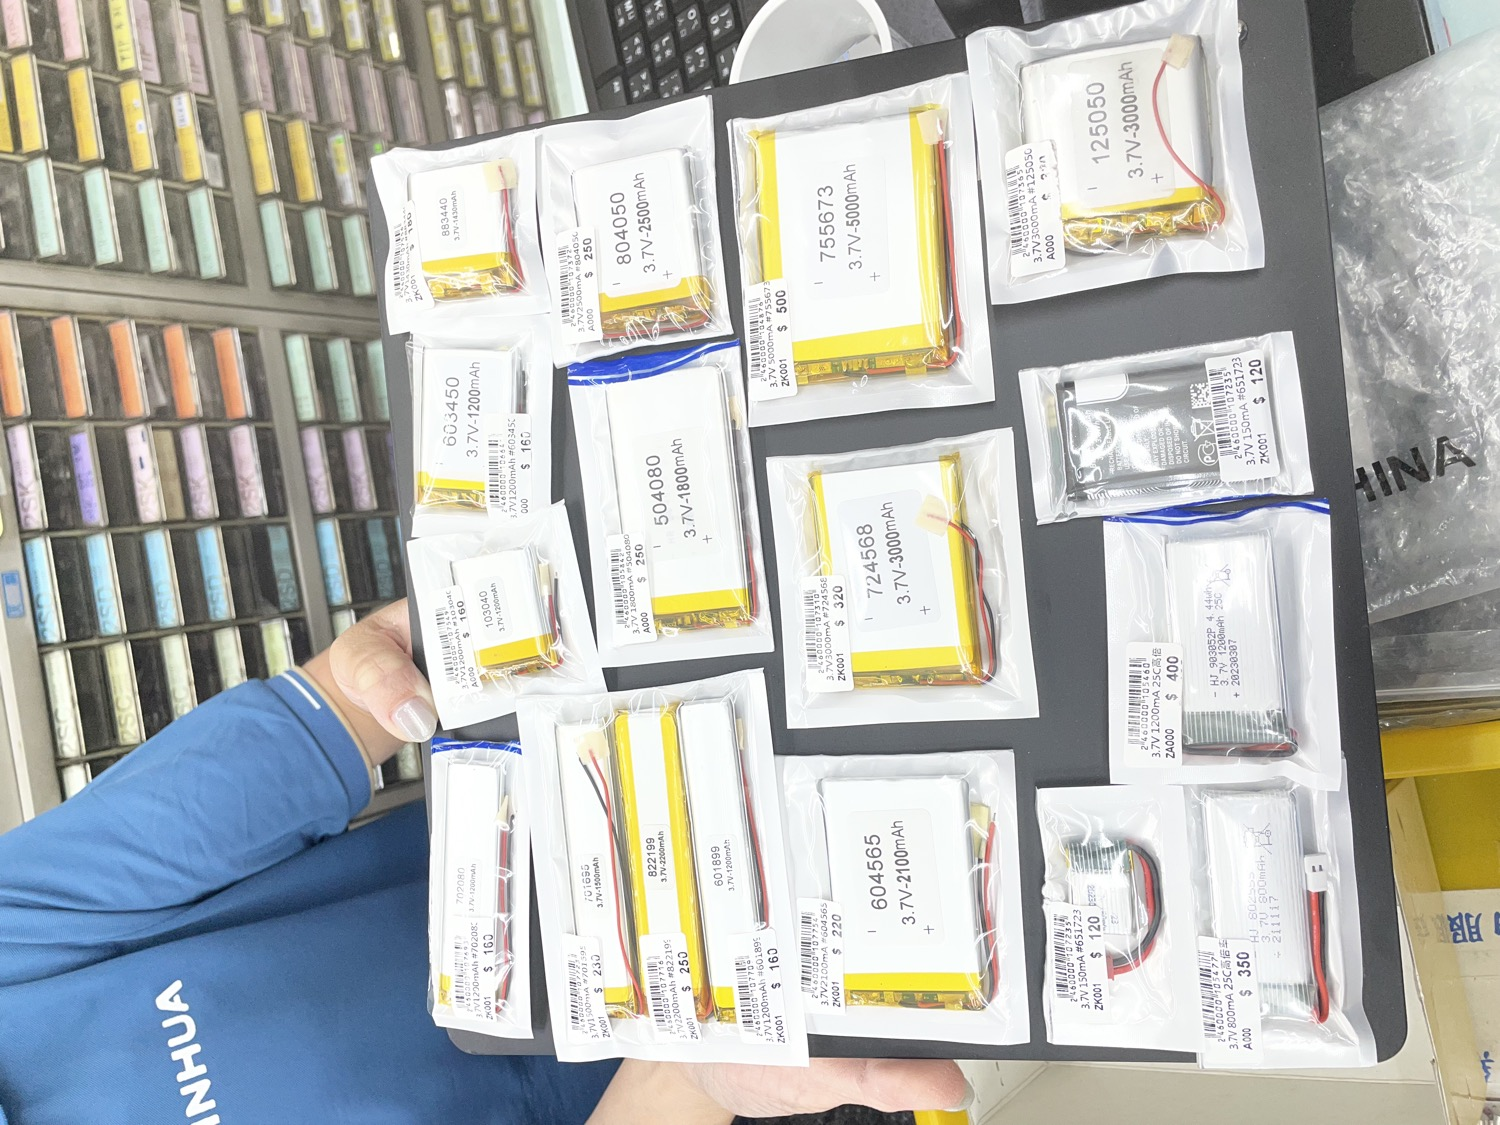
\includegraphics[width=0.55\linewidth]{2026-05-11/LiPo.jpg}
  \caption{今天買到的 3.7 V / 1200 mAh LiPo 電池(\#6034),
           回家拆袋後拍下實物存檔;原始 HEIC 留在
           \texttt{figures/2026-05-11/LiPo.HEIC}。}
  \label{fig:0511-lipo}
\end{figure}

\subsection*{今日心得}

\begin{itemize}[leftmargin=2em,itemsep=0pt]
  \item \textbf{今天最大的突破不是買到任何零件,而是發現 ADC 兩端的「dead zone」可以當訊號用}。
        原本以為要犧牲 \(\sim 18\%\) 的動態範圍,
        現在反過來看 \(\Rightarrow\) 那 18\% 就是免費的「該換檔」自動訊號。
        一個 \texttt{if v > 3.0: switch\_to\_lower\_gain()} 的迴圈,
        加 hysteresis 防抖,系統就比手轉旋鈕還聰明。
  \item \textbf{硬體界線一直在動}:4/19 時想用機械旋鈕,
        4/21 想著買波段開關沒買到,今天直接跳級到 mux + MCU 控制。
        每次重新想都比上次省一點手動操作,這就是迭代設計該有的方向。
  \item 0.3 V 跟 3.0 V 這兩個門檻數字得校準,有溫漂跟個體差,
        \textbf{下一步}:接上 74HC4051 量四檔的實際飽和點 + 底噪點,
        作為自動換檔狀態機的常數;同時下單 LDO(HT7133 或 XC6206-3.3V)
        把電池供電鏈補齊。
\end{itemize}


\logentry{2026-05-12}{Pico 焊接、最終電路定稿、決定 fork C++ 版本}
% =====================================================================
%  2026-05-12 — Pico 焊接、最終電路定稿、決定 fork C++ 版本
% =====================================================================

\subsection*{今日目標}

\begin{itemize}[leftmargin=2em,itemsep=0pt]
  \item 5/11 取的 \textbf{HS-02A 烙鐵}今天正式上戰場:
        \textbf{Pico 排針焊上}、\textbf{BPW34 焊成獨立長線},麵包板可以乾淨收線。
  \item 把 \textbf{74HC4051 MUX} 接到四檔 \(R_F\) (5/11 採購)、串到 op-amp 反相輸入、
        S0/S1 從 Pico GPIO 控,真正把「四檔自動換」這條線跑起來。
  \item 把整塊電路收成\textbf{最終定稿}:單一 Type-C 供電、OLED 接上、感測器與電路分離。
  \item 開始調 mux 自動換檔的 hysteresis 狀態機(5/11 那個 insight 的程式化)。
  \item \textbf{下一個分水嶺}:調著調著發現 MicroPython 採樣速度撐不住目標,
        正式 fork 一個 \textbf{C++ Pico SDK 版本}的 firmware 走下去。
\end{itemize}

\subsection*{第一個任務:焊接}

\paragraph{Pico 排針。} 5/11 採購的 Pico(20-pin \(\times 2\))出廠時排針是分離的;
今天用 HS-02A(C245 系統,330 \(^\circ\)C)把 40 隻腳焊上 \(\approx\) 15 分鐘搞定。
焊錫筆 \(\SI{1.0}{\milli\metre}\) 配無鉛助焊劑(松香膏),焊點圓潤、無短路。

\paragraph{BPW34 焊長線。} 5/6 量測的痛點之一是 BPW34 翹起來、貼不到螢幕。
今天用 \(\sim 30\) cm 帶絕緣的雙芯細線把 BPW34 與麵包板分開,
末端焊接點熱縮管包好(圖~\ref{fig:0512-bpw34}),BPW34 就能像「探棒」一樣\textbf{平貼螢幕}量測。

\begin{figure}[H]
  \centering
  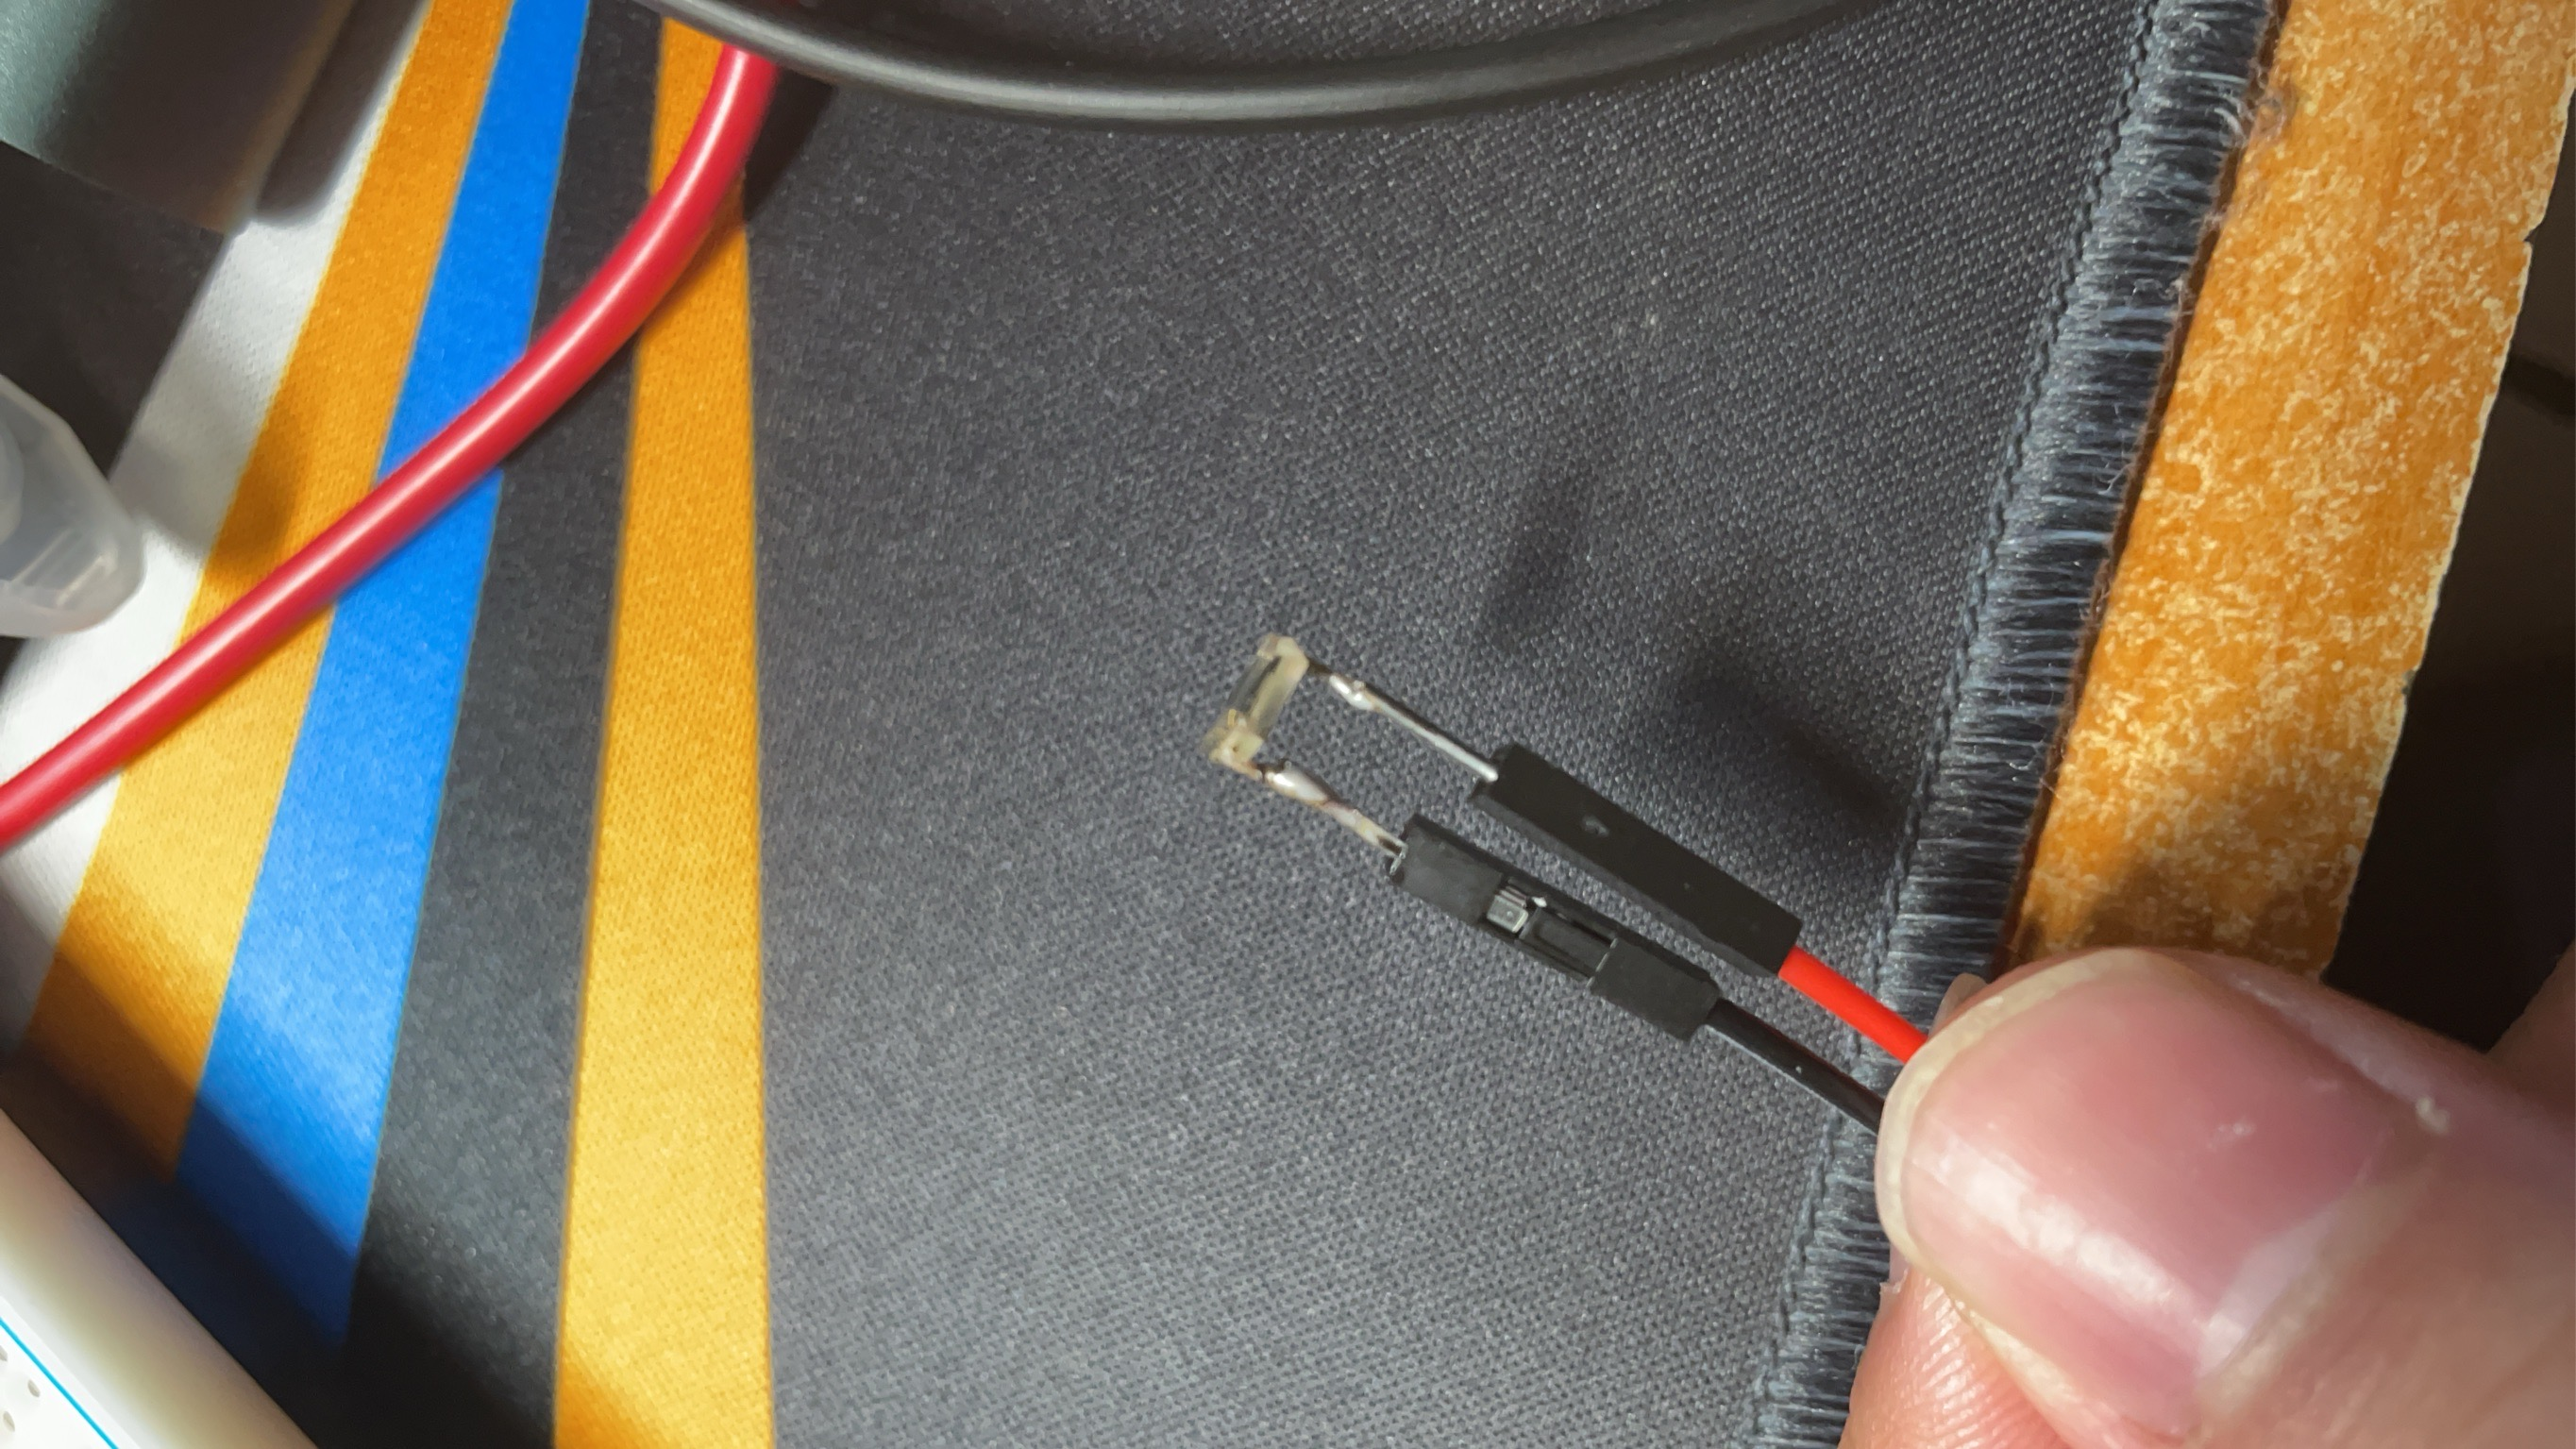
\includegraphics[width=0.55\linewidth]{2026-05-12/BPW34_solder.JPG}
  \caption{BPW34 焊到 30 cm 雙芯線末端,根部熱縮管固定,
           長線設計讓感測器可以離開麵包板平貼待測螢幕。}
  \label{fig:0512-bpw34}
\end{figure}

\subsection*{第二個任務:把 74HC4051 接到四檔 \(R_F\)}

5/11 從 Gemini 借來的拓樸今天落地:

\begin{itemize}[leftmargin=2em,itemsep=0pt]
  \item \texttt{COM}(Z 腳)接 op-amp 反相輸入(MCP6004 Pin 2)
  \item \texttt{Y0/Y1/Y2/Y3} 各接一支 \(R_F\):1 kΩ / 10 kΩ / 100 kΩ / 1 MΩ
  \item \(R_F\) 另一端統一拉到 op-amp 輸出(Pin 1)
  \item \texttt{S0/S1} 各接 Pico GPIO 一隻,\texttt{S2} 拉地(用不到第 5--8 通道)
  \item \texttt{INH}(enable, low-active)拉地長期開
\end{itemize}

\subsection*{第三個任務:電路最終定稿}

把零件擺位收成圖~\ref{fig:0512-final}的版本,有四個明顯升級:

\begin{enumerate}[leftmargin=2em,itemsep=2pt]
  \item \textbf{沒有杜邦線繞成一坨} —— 5/11 採購的 140 根預剪硬跳線終於發揮 ——
        所有走線水平貼板,目視能直接 trace 訊號流。
  \item \textbf{BPW34 從電路獨立出去} —— 透過上面那條 30 cm 長線拉出來,
        貼螢幕量測不會把整塊麵包板一起搬。
  \item \textbf{0.91" SSD1306 OLED 完整驅動} —— I\textsuperscript{2}C 兩線從 Pico 接出來,
        \texttt{firmware/python-version/ssd1306.py} (5/11 寫好) 直接吃。
  \item \textbf{全部單一 Type-C 供電} —— Pico 的 USB-C 同時兼任電源 + 資料線,
        9V 變壓器 + MB-102 退役(那兩件先留著當實驗室備援電源)。
\end{enumerate}

\begin{figure}[H]
  \centering
  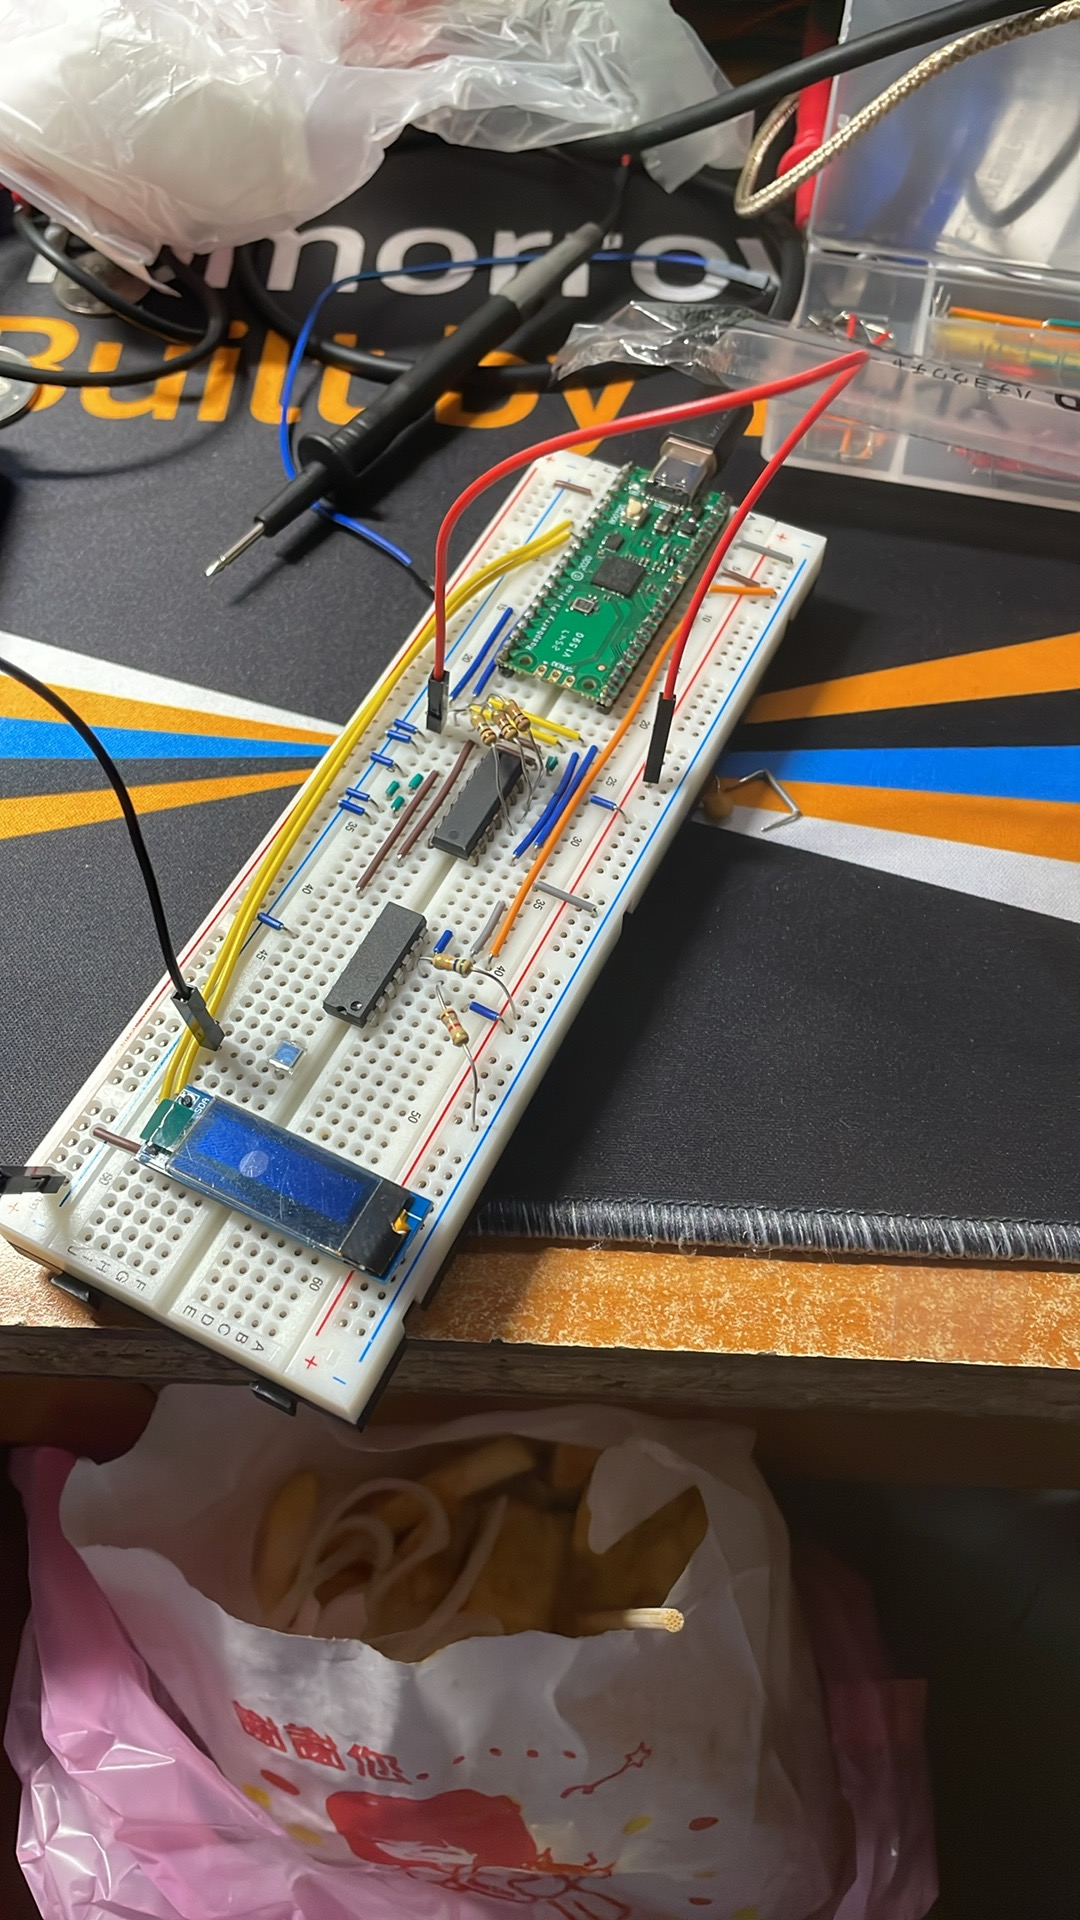
\includegraphics[width=0.85\linewidth]{2026-05-12/final_schmatic.JPG}
  \caption{2026-05-12 麵包板最終定稿:單 Type-C 供電(右下 Pico)、
           74HC4051 MUX + 四檔 \(R_F\)、MCP6004 TIA、SSD1306 OLED、
           BPW34 透過長線拉出畫面外平貼螢幕。}
  \label{fig:0512-final}
\end{figure}

\subsection*{第四個任務:hysteresis 自動換檔狀態機}

5/11 寫過構想了,今天程式化。MicroPython 端:

\begin{itemize}[leftmargin=2em,itemsep=0pt]
  \item 每 \(N\) 個樣本(目前 \(N = 100\),約 \(\SI{10}{\milli\second}\)) 算一次 mean。
  \item 若 mean \(> V_\text{HI} = \SI{2.8}{\volt}\) 連續 3 個視窗 \(\to\) 切下一檔較低 \(R_F\)。
  \item 若 mean \(< V_\text{LO} = \SI{0.5}{\volt}\) 連續 3 個視窗 \(\to\) 切下一檔較高 \(R_F\)。
  \item 切檔後 \(\SI{50}{\milli\second}\) cooldown(74HC4051 \texttt{tPHL}+RC settle 留 margin),
        cooldown 期間用 \texttt{print("\# GAP=...")} 通知 PC 端不要把這段當訊號。
\end{itemize}

實測:\textbf{會切,但切完抖一下}——cooldown 設太短 + MicroPython GC 時不時跳出來吃 50--100 ms,
換檔當下 PC 端能看到 burst-noise。可以調 cooldown 改善,但更基本的問題在後面那一節。

\subsection*{分水嶺:為什麼今天決定 fork C++ 版本}

調 mux 切檔時注意到幾個 MicroPython 撐不住的點:

\begin{itemize}[leftmargin=2em,itemsep=0pt]
  \item \textbf{ADC 取樣速率上限}:輪詢 \texttt{adc.read\_u16()} +
        \texttt{sys.stdout.write()} 兩件事就吃光 CPU,實測穩定上限 \(\approx \SI{8}{\kilo\hertz}\),
        距離 OLED PWM \(\SI{20}{\kilo\hertz}\) 要的 \(\geq 5 \times f\) Nyquist margin 不夠。
  \item \textbf{Jitter 大}:MicroPython runtime 不時 GC,\(\SI{50}{\micro\second}\) 級的 sample period
        會被偶發拉到 \(\SI{1}{\milli\second}\)+,FFT 出來有 sidelobe。
  \item \textbf{GAP marker 太頻繁}:OLED refresh、GC、切檔三個事件加起來,
        每秒會吐 5--10 個 GAP,PC 端拼時間軸要做太多 patch。
\end{itemize}

決定:\textbf{firmware 主線轉 C++ Pico SDK},用 PIO + DMA 把 ADC 取樣丟到 ring buffer,
GPIO 與 OLED I\textsuperscript{2}C 由 core1 慢工負責,采樣不再被任何 housekeeping 打斷。
MicroPython 版本保留在 \texttt{firmware/python-version/} 當原型參照,不丟。

\paragraph{cpp-version 目錄結構建好。}
\(\)同步把 C++ 兩個子專案的骨架擺進來,等接下來幾天慢慢長:

\begin{itemize}[leftmargin=2em,itemsep=0pt]
  \item \texttt{firmware/led-light-test-cpp-version/} —— C 版本的 blink
        (\texttt{blink.c} + \texttt{CMakeLists.txt} + \texttt{pico\_sdk\_import.cmake}),
        對應 python-version 的 blink.py;\textbf{確認 Pico SDK 編譯鏈通了}的基準起點。
  \item \texttt{firmware/cpp-version/} —— flicker meter 主程式 C++ 骨架
        (\texttt{main.cpp} + \texttt{ssd1306.cpp/.hpp} + 自家 SSD1306 OLED 驅動 +
        CMake build system)。今天先把目錄 + 起手檔 commit 起來,
        ADC PIO/DMA 那塊明後天動。
\end{itemize}

\subsection*{今日心得}

\begin{itemize}[leftmargin=2em,itemsep=0pt]
  \item \textbf{MicroPython 是好原型,但不是好量產}。功能完整跑通(blink \(\to\) ADC \(\to\) OLED \(\to\)
        mux \(\to\) 自動換檔)花了 4 天(5/8\,\(\to\)\,今天),效能瓶頸碰到要轉 C++ 也是 4 天。
        快速失敗才能快速知道接下來要走哪條路。
  \item \textbf{把語言版本當成資料夾並排}的設計(\texttt{python-version/} \(+\) \texttt{cpp-version/})
        現在看格外划算 —— python-version 不用刪、可繼續當原型 sandbox,cpp-version 主線重寫。
        日後甚至可以做兩版的同電路對比(同一 ADC 訊號 \(\to\) 兩個版本各跑 FFT \(\to\) 誰的 jitter 小)。
  \item \textbf{下一步}:
        \begin{enumerate}[leftmargin=2em,itemsep=0pt]
          \item C++ 端把 ADC \(\to\) PIO \(\to\) DMA \(\to\) ring buffer 那條鏈寫完,
                目標 \(\SI{100}{\kilo\hertz}\) 採樣率穩定無 jitter。
          \item OLED 從 C++ 端重新驅動(\texttt{ssd1306.cpp/.hpp} 已起手),
                跟 \texttt{firmware/python-version/ssd1306.py} 行為對齊。
          \item PC 端 \texttt{host/read\_data.py} 已能吃 binary 三 byte frame + GAP marker,
                C++ 版本只要照協定吐就能直接接,Host 不用動。
        \end{enumerate}
\end{itemize}


\logentry{2026-05-18}{設計第一版 PCB:PD\_detector\_pro (flico shield v1)}
% =====================================================================
%  2026-05-18 — 設計第一版 PCB:PD_detector_pro (flico shield v1)
% =====================================================================

\subsection*{今日目標}

\begin{itemize}[leftmargin=2em,itemsep=0pt]
  \item 把 5/12 麵包板上的「BPW34 \(+\) MCP6002 TIA \(+\) 74HC4051 mux \(+\) Pico \(+\) OLED」
        這條訊號鏈轉成 PCB——但是\textbf{先做 first-version,不是要直接投產}。
  \item 借這版 PCB 把 \textbf{KiCad/SKiDL 設計流程}走一遍:選 0805 SMD 規格、
        綁 LCSC 編號、SKiDL 跑出 netlist、KiCad 匯入 + 用 Python (\texttt{pcbnew})
        程式化擺件、輸出 Gerber/BOM/CPL。整套流程下次設計第二版時可以直接重用。
  \item 順便對\textbf{元件規格做一次升級盤點}:從麵包板的 hobby-grade
        (MCP6002, 74HC4051, Pico ADC) 升到精密量測等級
        (OPA328, TMUX1208, 外接 ADS8326 16-bit SAR),
        確認規格升上去後 PCB 該長什麼樣。
\end{itemize}

\subsection*{為什麼是 \texttt{first-version} 不是 \texttt{v1.0}}

幾個還沒收斂的關鍵問題,故意留給之後的版本解:

\begin{itemize}[leftmargin=2em,itemsep=0pt]
  \item \textbf{感測器選型}:雖然麵包板是用 BPW34(便宜、好買),但 0518 討論時意識到
        \textbf{SFH 2440}(更接近人眼響應、低反向暗電流)更適合做螢幕閃爍量測。
        但 SFH 2440 是 \emph{top-looker} SMD 封裝,感光面垂直 PCB 出來,
        跟「裝在耳機盒底部、光從底面進」的機構配置直接衝突 —— 要嘛走 90 度導光柱
        (3D 印透明 PETG/壓克力),要嘛改型號。今天的版本先沿用 BPW34
        把佈線跑通,選型留到 v2 收尾。
  \item \textbf{外殼方向}:「耳機盒」造型(USB-C 朝上、感光口朝下、Pico 與 PCB 平行疊)
        的機構決策今天才定下來,3D 列印外殼還在 Fusion 360 裡半成品。
  \item \textbf{ADC 軟體鏈}:把採樣率拉到 \(\SI{32}{\kilo\hertz}\) 要靠 Pico 端
        SPI \(+\) hardware timer \(+\) USB binary stream,這條鏈得用 C++ Pico SDK
        重寫(5/12 已決定),但今天 host 端的 PyQtGraph dashboard 也還沒寫。
  \item \textbf{電池供電}:原本想做 LiPo 內建,但 OPA328 \(+\) TMUX1208 \(+\) ADS8326
        全要 \(\SI{3.3}{\volt}\) 純淨類比電源,USB 雜訊問題用 ferrite bead \(+\) LP5907 LDO
        解。電池路徑加上 MCP73831 充電 IC \(+\) SS14 蕭特基 OR-ing,目前已畫入 schematic
        但實體尚未在麵包板驗證,可能 v2 就把整段砍掉、改純 USB 供電。
\end{itemize}

所以這版定位是\textbf{流程驗證 + 規格盤點}:讓 SKiDL/pcbnew 工具鏈跑通,
把元件升級的影響真實畫到佈線上看,但不送 JLCPCB 投產。\textbf{歸檔在
\texttt{hardware/first-version/}。}

\subsection*{規格升級盤點}

對照麵包板原型(5/12 定稿)→ 這版 PCB:

\begin{table}[H]
  \centering
  \caption{flico 從麵包板原型升級到 first-version PCB 的元件規格盤點。}
  \label{tab:0518-spec}
  \small
  \begin{tabular}{lll}
    \toprule
    位置 & 麵包板版本 & first-version PCB 版本 \\
    \midrule
    Op-amp     & MCP6002 (DIP-8, 100\,pA $I_B$)
               & \textbf{OPA328} (SOT-23-5, 0.2\,pA $I_B$, RRIO, 3.3\,V) \\
    類比 mux   & 74HC4051 (8-ch, $R_\text{on}$\,$\approx$\,100\,\(\Omega\), \(I_\text{leak}\) ns\,nA)
               & \textbf{TMUX1208} (8-ch, $R_\text{on}$\,$\approx$\,5\,\(\Omega\), \(I_\text{leak}\) ns\,10\,pA) \\
    回授網路   & 4 檔 (1\,k / 10\,k / 100\,k / 1\,M)
               & \textbf{8 檔對數} (1\,k, 3.3\,k, 10\,k, 33\,k, 100\,k, 330\,k, 1\,M, 10\,M\(\Omega\)) \\
    回授補償 $C_f$ & 雜湊配對(1\,n / 330\,p / 33\,p / 1\,p)
               & 全部按 \(f_c=\SI{16}{\kilo\hertz}\) 重算:10\,n / 3.3\,n / 1\,n / 330\,p / 100\,p / 33\,p / 10\,p / 1\,p \\
    ADC        & Pico 內建 (12-bit, ENOB $\approx$ 9, 跟著數位雜訊)
               & \textbf{ADS8326} (外接 SPI, 16-bit SAR, 250\,kSps) \\
    電源       & Pico 3V3 直接餵類比
               & VBUS \(\to\) ferrite bead \(\to\) \textbf{LP5907} LDO \(\to\) +3V3\_A (類比專屬軌) \\
    接地       & 單一 GND
               & \textbf{Star grounding}:GND \(+\) GNDA 分離,LDO 旁邊 0\,\(\Omega\) 拼回 \\
    電池       & 不接(5/11 LiPo 還沒上)
               & MCP73831 充電 + SS14 OR-ing(畫進去但 v2 可能砍) \\
    顯示       & SSD1306 0.91" OLED via I\textsuperscript{2}C
               & 同上(複用 5/11 寫好的 \texttt{ssd1306.py}) \\
    \bottomrule
  \end{tabular}
\end{table}

關鍵理由:

\begin{itemize}[leftmargin=2em,itemsep=0pt]
  \item \textbf{OPA328 取代 MCP6002}:在 10\,M\(\Omega\) 高增益下,
        100\,pA 偏置電流會在輸出端疊出 \(\SI{1}{\milli\volt}\) 偏置 + 漂移;
        0.2\,pA 直接降 500 倍,基本上是測量極限的天花板。
  \item \textbf{TMUX1208 取代 74HC4051}:
        \(R_\text{on}\) 從 100\,\(\Omega\) 降到 5\,\(\Omega\),在 1\,k\(\Omega\) 檔位的增益誤差
        從 10\% 降到 0.5\%;漏電流降 100 倍,10\,M\(\Omega\) 檔位的偏置誤差從
        \(\sim 10\,\mathrm{mV}\) 降到不到 \(\SI{1}{\micro\volt}\)。
  \item \textbf{8 檔對數 \(R_f\)}:1\(\to\) 10 跳階(4 檔)會在中間出現
        「上一檔太弱、下一檔已飽和」的死區;改 \(1 \to 3.3 \to 10\) (E12 序列、8 檔)
        可以無縫覆蓋 \(10^7\) dynamic range,自動換檔的 hysteresis 變得更平順。
  \item \textbf{每檔 \(C_f\) 按 \(f_c = \SI{16}{\kilo\hertz}\) 收歛}:
        \(C_f = 1 / (2\pi f_c R_f)\)、目標 Nyquist 截止跟採樣率對齊。
        從原本「能塞什麼塞什麼」改成正規 anti-alias filter,所有檔位的頻寬都對齊在
        \(\sim \SI{16}{\kilo\hertz}\),量測一致性提升。
  \item \textbf{外接 ADS8326 取代內建 ADC}:RP2040 內建 ADC 的 INL/DNL 鋸齒誤差
        已知會把 ENOB 拉到 \(\sim 9\) bit,加上跟 Pico 數位電路共電的雜訊,
        12-bit 名義上的精度根本拿不到;外接 16-bit SAR 直接給乾淨的 65,536 階。
  \item \textbf{LP5907 LDO + ferrite bead + 星型接地}:
        Pico 的 3V3 是 buck 出來的、有 \(\sim \mathrm{kHz}\) ripple;
        要做精密類比就得有一條獨立的、跟數位地解耦的 +3V3\_A。
\end{itemize}

\subsection*{設計流程:SKiDL \(\to\) Netlist \(\to\) KiCad \(\to\) Python \texttt{pcbnew} 自動擺件}

KiCad 8/10 的原生流程是 GUI:在 Schematic Editor 拉線、annotate、選 footprint、
按 F8 (\emph{Update PCB from Schematic})、在 PCB Editor 手動擺件。今天決定走 \textbf{程式化}
路線,理由是:這版會反覆改規格,GUI 重畫很煩、版本控制(看 diff)也痛苦。

\begin{itemize}[leftmargin=2em,itemsep=0pt]
  \item \textbf{Schematic}:用 \textbf{SKiDL}(Python DSL for schematics)寫\\
        \texttt{hardware/first-version/gen\_schematic.py}。元件用 \texttt{Part("Device", "R", ...)}
        宣告,連線用 Python \texttt{Net} 物件 \texttt{+=}。
        產出 \texttt{pd\_detector.net}(KiCad netlist 格式)。
  \item \textbf{Footprints 綁 LCSC}:SKiDL 元件加自定義欄位
        \texttt{LCSC=Cxxxxx} 直接寫進 BOM(56k 0805 \(\to\) C17414、
        SS14 \(\to\) C8601、MCP73831 \(\to\) C116490 …… ),
        JLCPCB 下單時不會問「這是哪一顆」。
  \item \textbf{Import 到 KiCad}:在 PCB Editor → \emph{File} → \emph{Import} → \emph{Netlist},
        指 \texttt{pd\_detector.net}。所有元件 footprint 一次跑到畫布,
        ratsnest(白色飛線)就是設計連線的全部 ground truth。
  \item \textbf{擺件靠 \texttt{pcbnew} Python API}:寫
        \texttt{hardware/first-version/apply\_layout.py},
        用座標把元件 一顆顆 \(\texttt{SetPosition(VECTOR2I\_MM(x, y))}\),
        透過 KiCad 內建的 Python 直譯器執行
        (路徑:\texttt{/Applications/KiCad/KiCad.app/Contents/Frameworks/Python.framework/.../python3})。
        改一個座標 \(\to\) 跑一次腳本 \(\to\) KiCad GUI \emph{Reload from Disk} \(\to\) 看結果,
        比拖 GUI 快 5\(\times\) 以上,而且版本控制看得到 diff。
  \item \textbf{rendering 出圖}:寫 \texttt{reset\_routing.py} 把線清乾淨重畫;
        SVG/PNG 渲染存在 \texttt{layout\_renders/} 給日記引用(圖~\ref{fig:0518-top-tia}~\ref{fig:0518-top}~\ref{fig:0518-island})。
\end{itemize}

\subsection*{關鍵架構決策:flipped analog island}

排到一半 Claude Code 跑出個 plan,把 D1(BPW34/SFH 2440)搬到 PCB 最下緣(\(Y=48.5\) mm,
靠近耳機盒底部光口),但把 TIA 那一塊(U2 OPA328、U3 TMUX1208、八檔 \(R_f / C_f\))留在板子中間(\(Y \approx 19.5\) mm)。我覆盤了一下,這個排法\textbf{表面合理但物理上致命}:

\begin{itemize}[leftmargin=2em,itemsep=0pt]
  \item \texttt{TIA\_SUM} net(光二極體陰極 \(\to\) op-amp \(V^-\))會橫跨 PCB 接近 30 mm。
  \item 在 \(R_f = 10\,\mathrm{M}\Omega\) 的高增益下,這 30 mm 銅箔就是一根超級天線,
        \(\SI{60}{\hertz}\) 市電雜訊會被吸進去放大七位數倍。
  \item Trace 自帶 \(\sim 0.5\,\mathrm{pF/cm}\) 寄生電容 \(\Rightarrow\) 30 mm \(\approx\) 1.5 pF \(\Rightarrow\)
        \(R_f = 10\,\mathrm{M}\Omega\) 那檔頻寬從 \(\SI{32}{\kilo\hertz}\) 掉到 \(\SI{25}{\kilo\hertz}\),
        甚至誘發 op-amp 震盪(因為 \(C_\text{in} + C_\text{parasitic}\) 超過相位 margin)。
\end{itemize}

對策:整塊\textbf{類比 island 一起翻到板底},D1 跟 TIA 貼緊放(\(Y = 35 \sim 48\) mm),
數位 ADC + decoupling 移到上半板(\(Y = 5 \sim 30\) mm)。\texttt{TIA\_SUM} 走線
壓到 \(\sim 3\) mm。代價是 SPI 那邊 trace 變長,但 SPI 是數位邏輯訊號、
雜訊容忍度高得多,完全可以接受。

\begin{figure}[H]
  \centering
  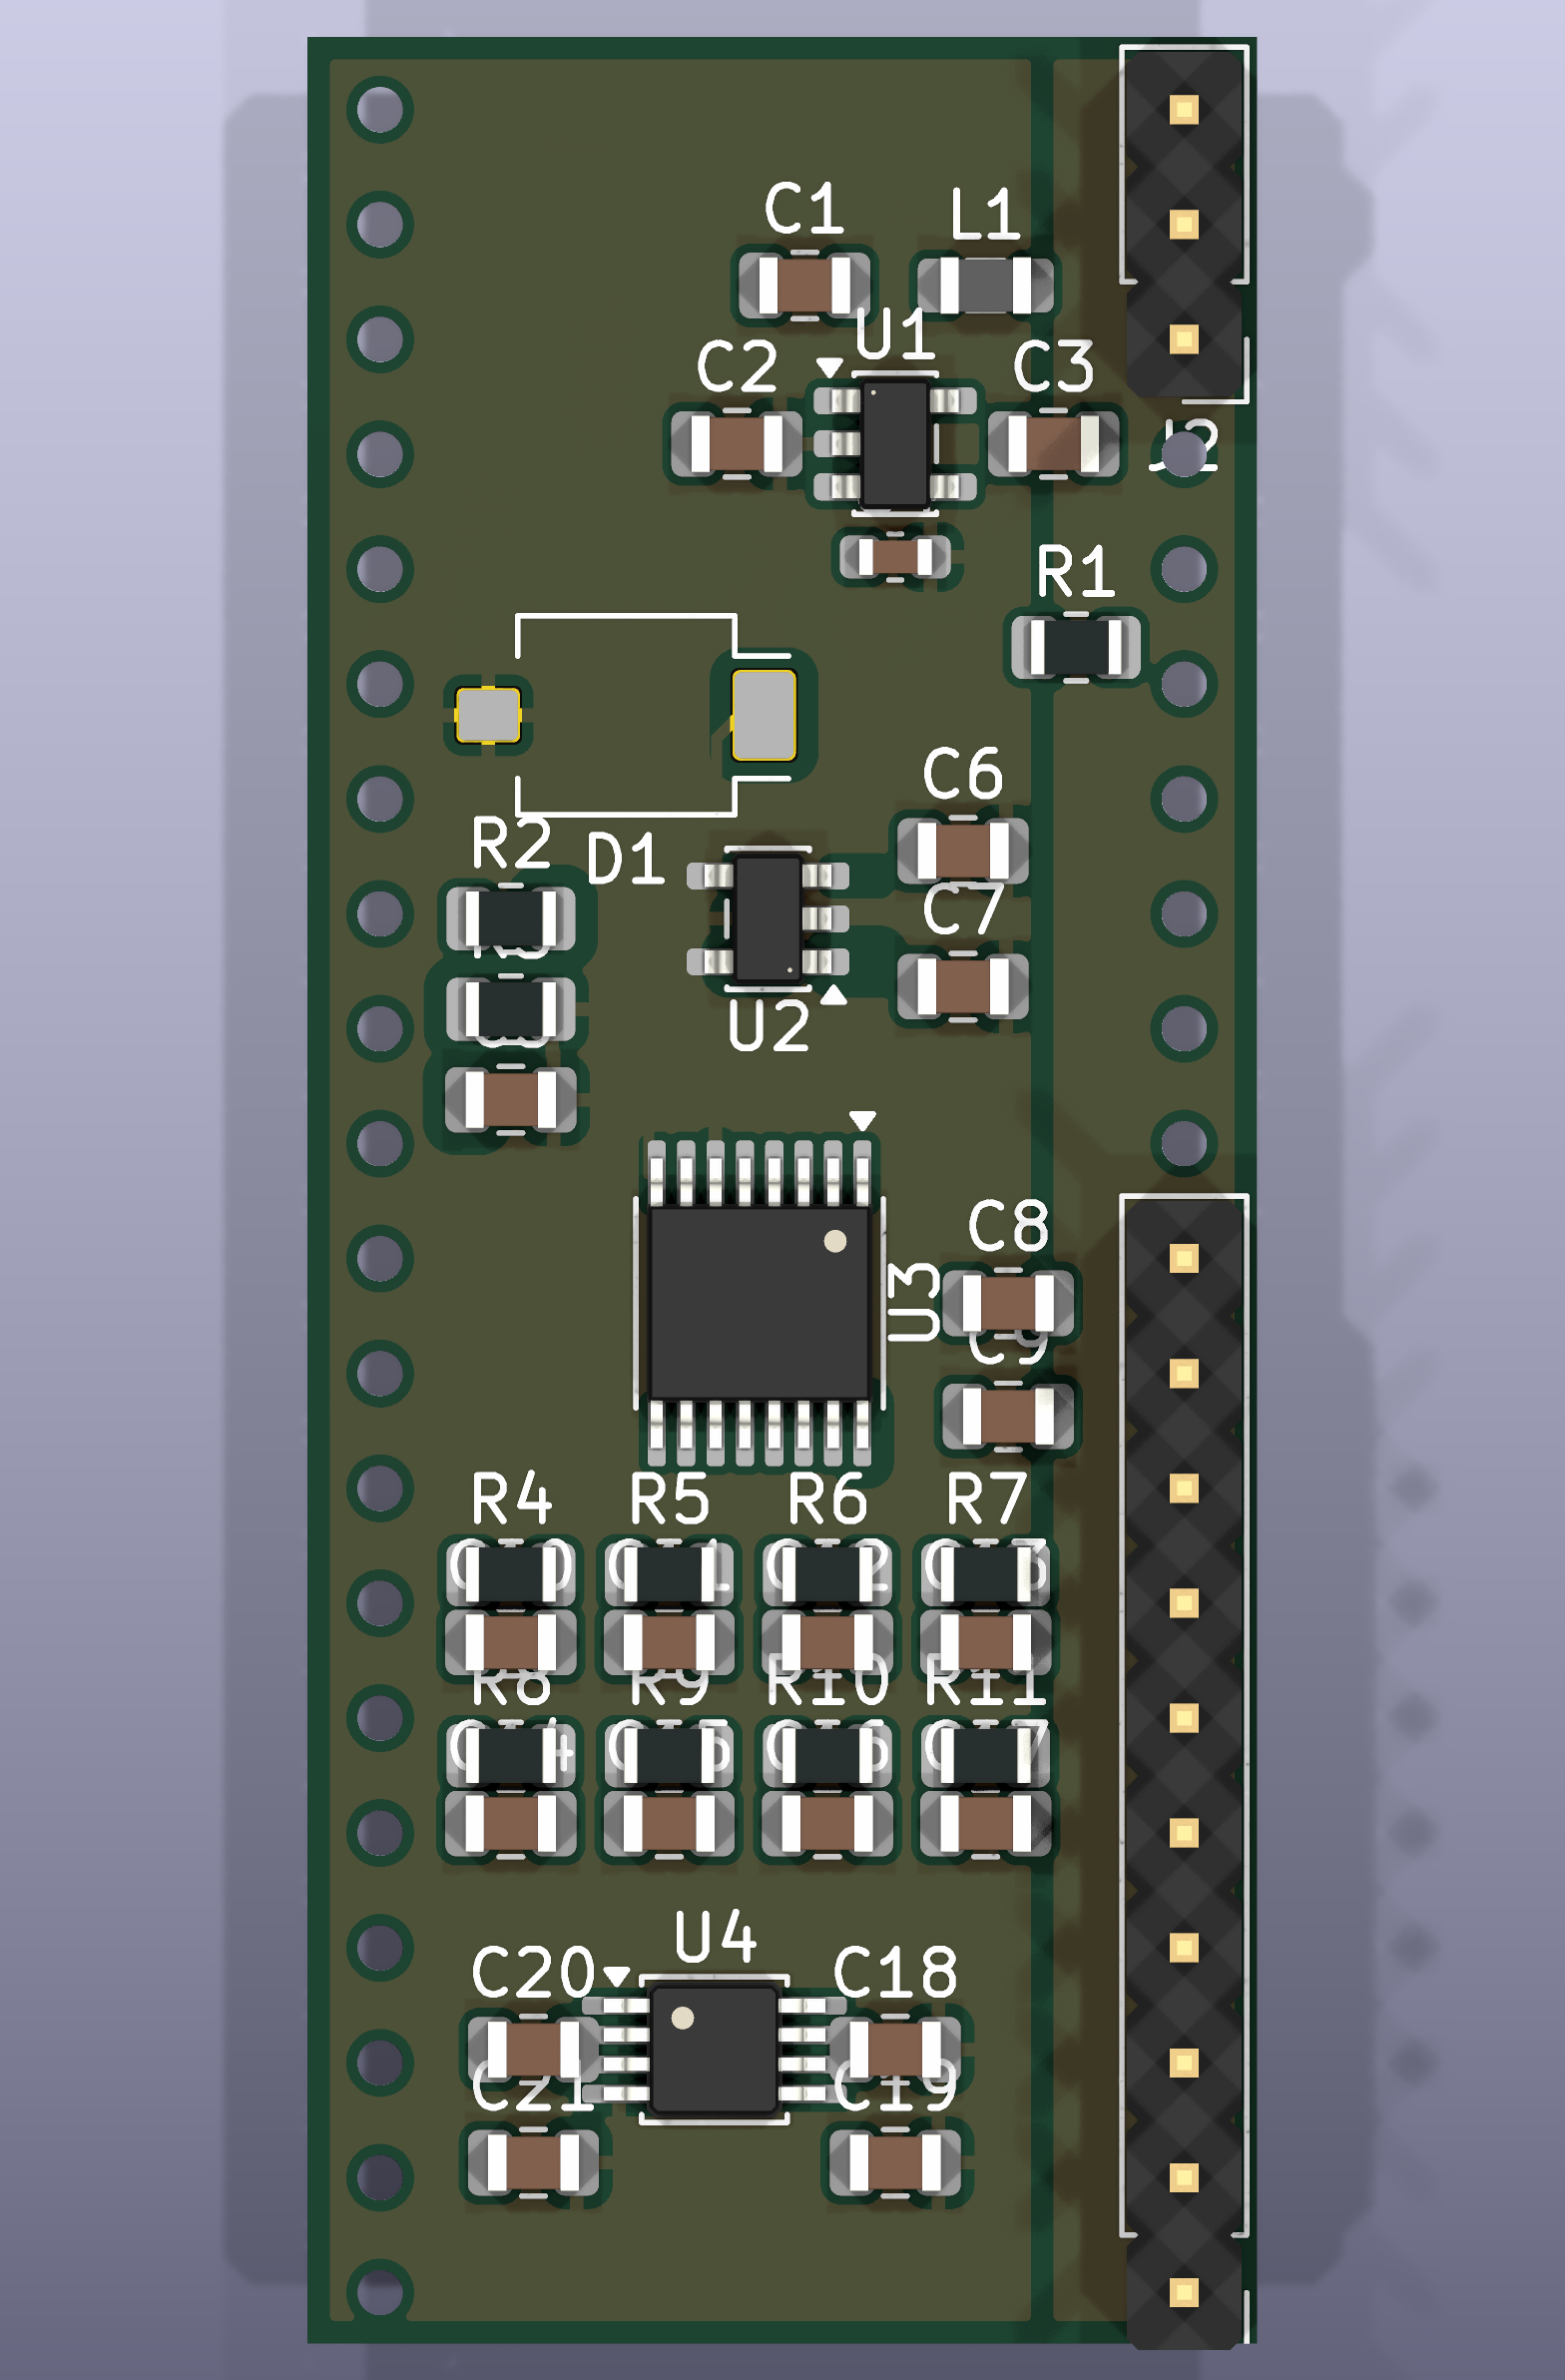
\includegraphics[width=0.7\linewidth]{2026-05-18/top_tia_sum.png}
  \caption{TIA 區塊放大渲染(top.svg 局部):op-amp(U2)、TMUX1208(U3)、
           八檔 \(R_f / C_f\) 全部緊靠 D1,\texttt{TIA\_SUM} 走線壓到 \(< 5\) mm。
           feedback 電容 \(C_f\) 跟 \(R_f\) 同點接,
           anti-alias filter 形成一致的 \(\sim \SI{16}{\kilo\hertz}\) 截止。}
  \label{fig:0518-top-tia}
\end{figure}

\begin{figure}[H]
  \centering
  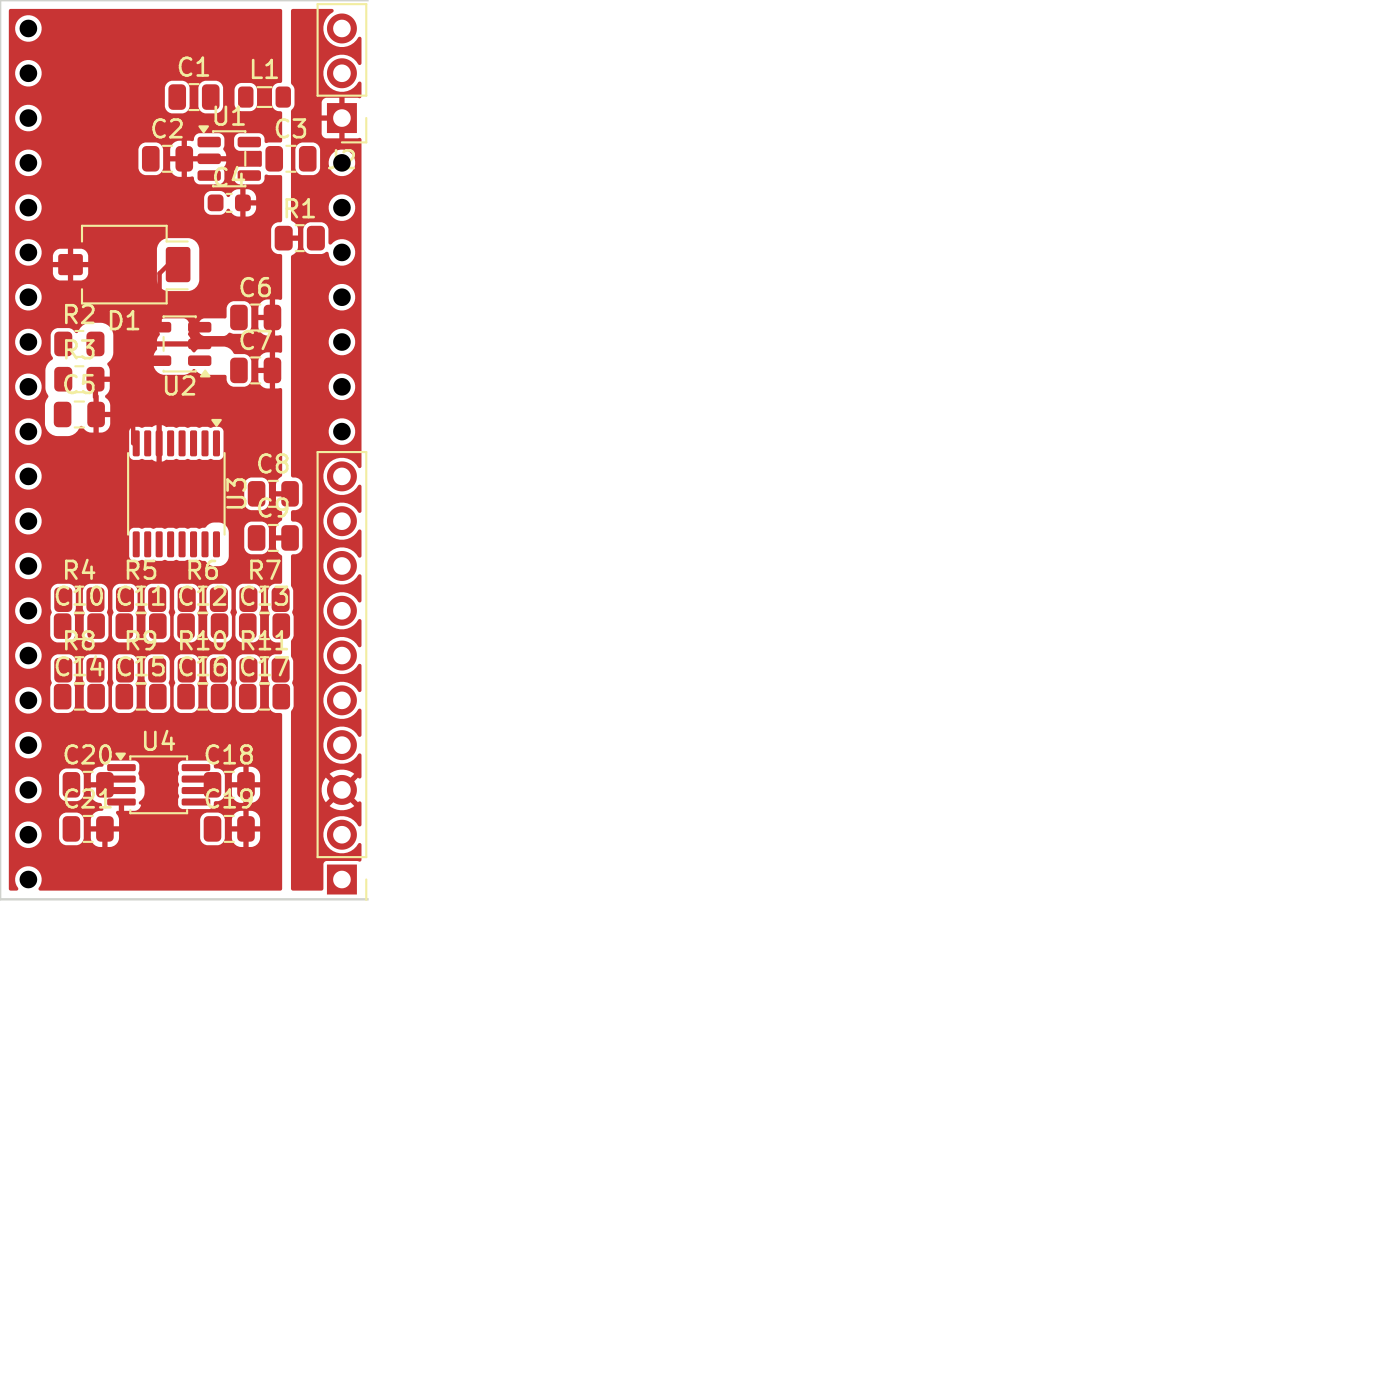
\includegraphics[width=0.85\linewidth]{2026-05-18/top.svg.png}
  \caption{flipped island 架構全板正面渲染。下半:類比安靜區(BPW34 D1
           + OPA328 TIA + TMUX1208 mux + 八檔 \(R_f / C_f\) + V\_REF 偏壓分壓)。
           上半:數位區(LP5907 LDO + ADS8326 SPI ADC + Pico header + MCP73831 充電)。
           中段 0\,\(\Omega\) 拼接點 = star ground,GND 跟 GNDA 在這唯一相連。}
  \label{fig:0518-top}
\end{figure}

\begin{figure}[H]
  \centering
  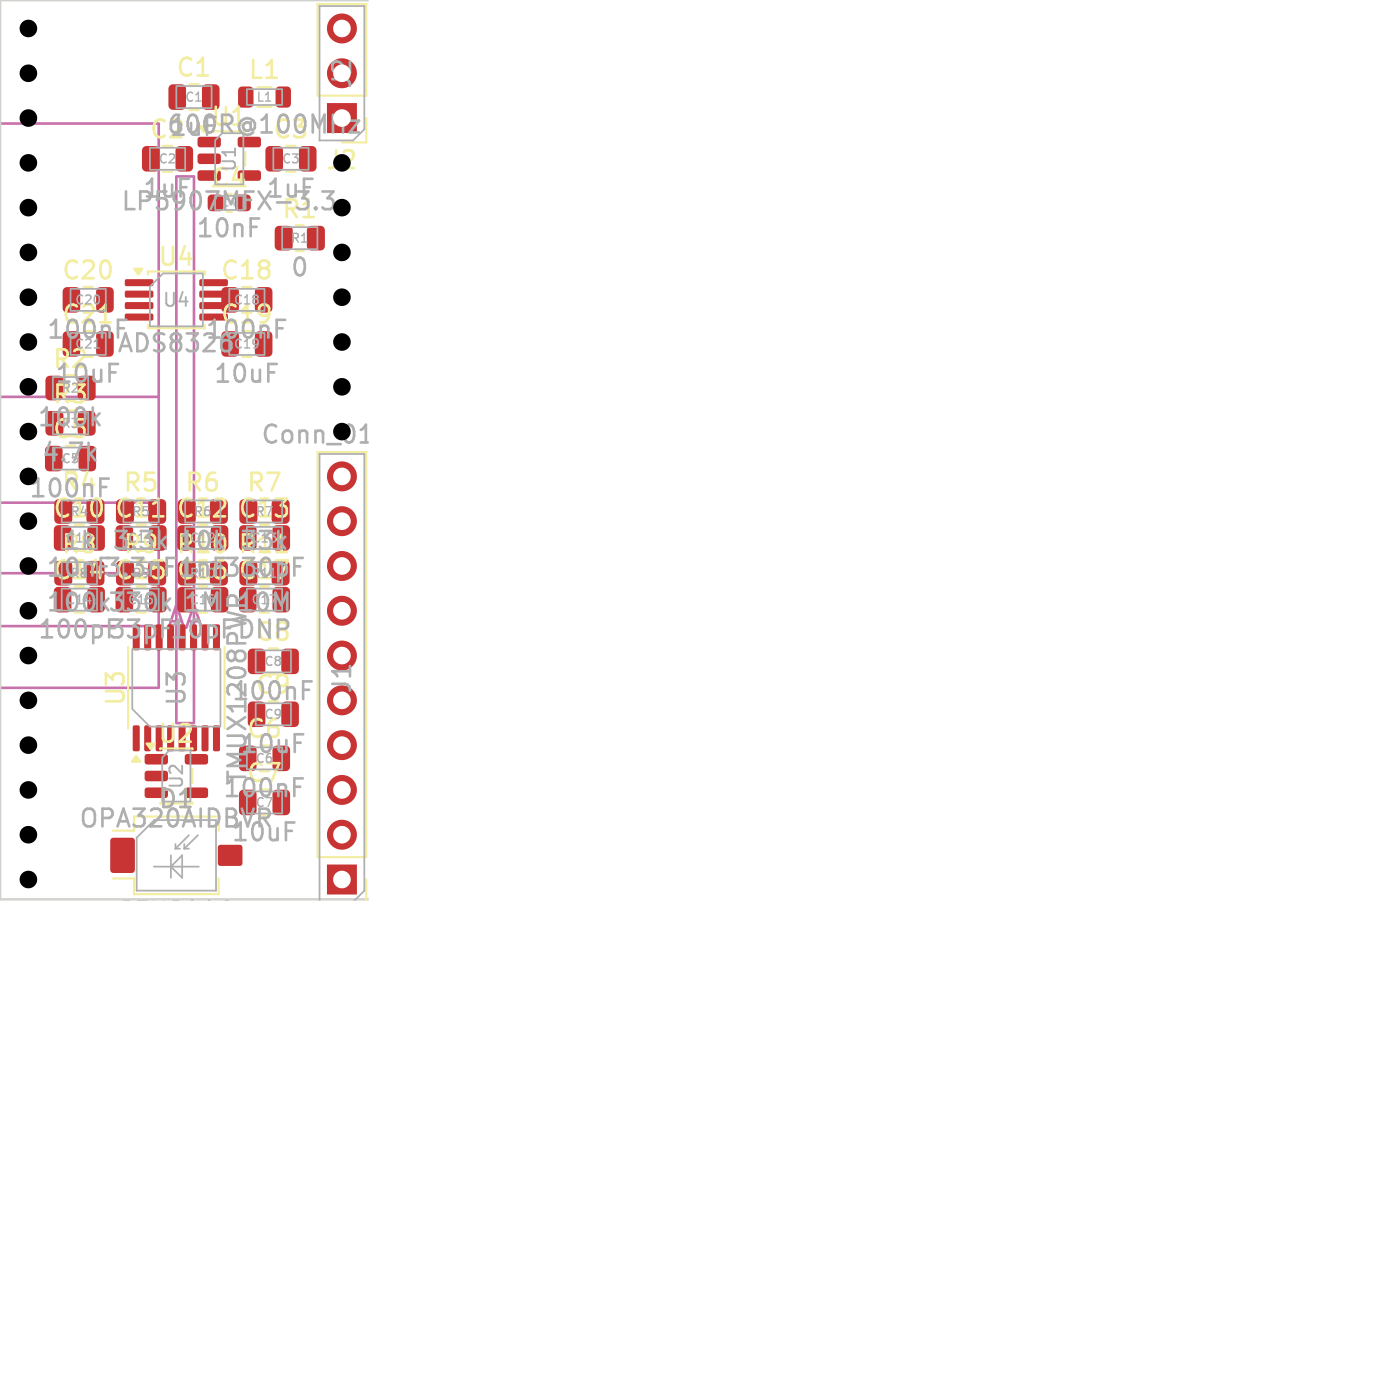
\includegraphics[width=0.7\linewidth]{2026-05-18/flipped_island.svg.png}
  \caption{flipped island 配置示意:把 D1(光感)從上方搬到下方,
           整塊 TIA 跟著翻轉,讓 \texttt{TIA\_SUM} 走線縮到最短。
           原本「ADC 在下、TIA 在上」是配合 USB-C/Pico 走線方便,
           但物理上犧牲了類比 SNR。}
  \label{fig:0518-island}
\end{figure}

\subsection*{順手解掉的細節}

過程中還塞了好幾個 0518 跟 Gemini/Claude 來回討論時學到的東西:

\begin{itemize}[leftmargin=2em,itemsep=0pt]
  \item \textbf{C0G/NP0 陶瓷材質}:八檔 \(C_f\) 都要 C0G/NP0,
        \textbf{不能用 X7R/Y5V} —— 後者有壓電效應,外殼震動會在 10\,M\(\Omega\)
        高增益下被放大成雜訊。
  \item \textbf{Mux common 接 \(V^-\) 不接 \(V_\text{out}\)}:把 TMUX1208 的 COM 接到
        op-amp 反相輸入(虛擬接地點)而非輸出端 —— 因為 mux 內部約 25 pF 寄生電容,
        如果掛在輸出端,會隨著 \(V_\text{out}\) 大幅充放電產生失真;掛在虛擬接地點電位幾乎不變,
        雜訊影響最小。
  \item \textbf{Power path}:USB \(\to\) D2 蕭特基 \(\to\) Pico VSYS;
        Battery \(\to\) D4 蕭特基 \(\to\) Pico VSYS;
        兩條 OR-ing。MCP73831 的 PROG 腳要 2\,k\(\Omega\) 到 GND 設充電電流 \(\sim 500\) mA。
        STAT 是 open-drain,LED 要接到 VBUS 上 \(\to\) 電阻 \(\to\) LED \(\to\) STAT,不能反過來。
  \item \textbf{ERC PWR\_FLAG}:KiCad ERC 會把
        \emph{Input Power pin not driven by any Output Power pins} 紅標出來。
        要在 VSYS 跟 GND/GNDA 各接一個 PWR\_FLAG,跟它說「這條線是真的有電的」。
  \item \textbf{打 via 規則}:\texttt{TIA\_SUM} 絕對不打 via(via 自帶 \(\sim 0.3\) pF 寄生 +
        阻抗不連續,10\,M\(\Omega\) 高增益下會放大);電源跟 GNDA 可以多打、
        孔徑也可以大(0.4 mm drill / 0.8 mm size)降低迴路阻抗。
\end{itemize}

\subsection*{產物 \(+\) 留檔}

當天的設計 commit 到 \texttt{hardware/first-version/}:

\begin{itemize}[leftmargin=2em,itemsep=0pt]
  \item \texttt{gen\_schematic.py}(\(\sim 300\) 行,SKiDL DSL) + \texttt{gen\_schematic\_sklib.py}
        (cache 的元件 symbol)
  \item \texttt{pd\_detector.net}(40 KB,KiCad netlist 格式 — schematic 的 ground truth)
  \item \texttt{PD\_detector\_pro.kicad\_pro / .kicad\_pcb / .kicad\_sch / .kicad\_prl}
        (PCB editor 專案;\texttt{.kicad\_sch} 是空 stub,因為 schematic 由 SKiDL 直接生 netlist,
        沒有 GUI schematic)
  \item \texttt{apply\_layout.py}(\(\sim 600\) 行,pcbnew API 程式化擺件) +
        \texttt{reset\_routing.py}(\(\sim 200\) 行,清線重畫)
  \item \texttt{gen\_schematic.erc / .log}(SKiDL 跑出來的 ERC 報告)
  \item \texttt{layout\_renders/}(top.svg / .png、flipped\_island.svg / .png、top\_tia\_sum.png)
\end{itemize}

\textbf{完整的 0518 Gemini 對話檔}留在
\texttt{report/research-log/gemini\_discuss\_history/0518.txt}(\(\sim 5000\) 行)——
從 0805 封裝選型、JLCPCB PCBA 流程、MCP73831 vs TP4056、LiPo 採購、I\textsuperscript{2}C OLED、
74HC4051 接線、SKiDL 跟 KiCad 整合、TMUX1208/OPA328/ADS8326 升級、抗混疊濾波公式、
flipped island 決策一路討論到 via 規則,完整重現整天設計思路。

\subsection*{今日心得}

\begin{itemize}[leftmargin=2em,itemsep=0pt]
  \item \textbf{先把流程跑通比先把規格定死重要}。元件選 OPA328 還是 OPA140、
        電池要不要進、SFH 2440 還是 BPW34,這些今天都沒最終定案 ——
        但 SKiDL \(+\) pcbnew Python API 這條\textbf{自動化設計流程}先跑通,
        下次改規格就只改幾行 Python,不用重新滑滑鼠拖 GUI。
  \item \textbf{flipped island 是今天最大的 architectural insight}。如果直覺照「Pico 朝上、
        D1 朝下」排,TIA 會掛在中間 \(\to\) \texttt{TIA\_SUM} 30 mm \(\to\) 板子當天線。
        類比設計的鐵律就是「敏感的東西盡量短盡量靠近」,要為了這個翻整塊 island 也得翻。
  \item \textbf{SKiDL 的最大好處不是寫起來快,是 review 起來快}。Schematic 變成 Python code,
        \texttt{git diff} 就能看見「上次到這次改了哪一條 net、加了哪顆元件」。
        對於 \textbf{Gemini/Claude 來回提案修改}的 workflow,文字 diff 不可或缺。
  \item \textbf{下一步}:
        \begin{enumerate}[leftmargin=2em,itemsep=0pt]
          \item \textbf{不打板。} 規格還沒收斂,直接送 JLCPCB 等於燒錢。
                把所有「待解」項目(感測器選型、SFH 2440 機構問題、電池要不要進、
                C++ ADC 鏈)各自獨立解掉,再做 v2。
          \item C++ firmware 主線(5/12 fork 出來那條)繼續推:
                ADC + PIO + DMA \(\to\) ring buffer,目標 \(\SI{32}{\kilo\hertz}\) jitter-free。
          \item Host 端 \texttt{host/} 寫 PyQtGraph 即時 dashboard,
                吃 USB binary stream + FFT + 自動跟著 Pico 的 GAP marker。
          \item 開始畫 3D 列印外殼(Fusion 360),確認 SFH 2440 光路要走導光柱
                還是側焊 — 機構決定回頭影響感測器選型。
        \end{enumerate}
\end{itemize}


\logentry{2026-05-19}{host 從 Python (matplotlib \(\to\) PyQtGraph) 改寫成 Rust}
% =====================================================================
%  2026-05-19 — host 端從 Python (matplotlib → PyQtGraph) 改寫成 Rust
% =====================================================================

\subsection*{今日目標}

\begin{itemize}[leftmargin=2em,itemsep=0pt]
  \item 解掉 host 端\textbf{即時繪圖卡頓}的問題:量測時間一拉長(累積樣本超過 \(\sim 3 \times 10^4\) 點)
        就掉到 \(\sim 0.5\) fps,根本看不到即時波形。
  \item 把 \texttt{host/} 從 Python 換掉。這幾天連續迭代過兩版
        (\texttt{matplotlib} \(\to\) \texttt{PyQtGraph})都沒能徹底解決效能,
        今天決定整個重寫成 \textbf{Rust}(\texttt{eframe} \(+\) \texttt{egui} \(+\) \texttt{egui\_plot})。
  \item 順手把 Rust 版做成\textbf{雙目標 build}:原生(macOS/Windows)+ WASM
        (\texttt{cargo run --target wasm32-unknown-unknown}),
        讓之後分享給同學看波形時直接開瀏覽器、不用 install。
\end{itemize}

\subsection*{Python 版的兩階段失敗}

\paragraph{階段一(5/8 \(\sim\) 5/12 用過):\texttt{matplotlib} + \texttt{plt.ion()} 互動模式。}
寫起來最快:

\begin{itemize}[leftmargin=2em,itemsep=0pt]
  \item \texttt{pyserial} 開 \texttt{/dev/cu.usbmodemXXX} \(\to\) 阻塞讀一行 \(\to\)
        \texttt{ax.lines[0].set\_data(...)} \(\to\) \texttt{plt.pause(0.01)}。
  \item \textbf{問題}:畫面\textbf{會閃}。每次 \texttt{plt.pause()} 內部 \texttt{draw\_idle()}
        會把整個 figure backend 重畫一次,在 macOS retina \(+\) Apple Silicon 上
        \(\sim \SI{60}{\hertz}\) 同步翻轉,畫到一半的 frame 會被推到螢幕 \(\Rightarrow\) 整條波形
        看起來像 PWM 一樣閃黑。把 \texttt{plt.pause} 拉到 \texttt{0.05} 改善了一點,
        但代價是 frame rate 直接掉到 \(\SI{20}{fps}\)。
  \item \textbf{根本原因}:matplotlib 的設計是「\textbf{出版品質靜態圖}」,不是「即時 oscilloscope」。
        backend(macOS 上 默認是 \texttt{macosx})每次 redraw 都重新計算 ticks、layout、字體
        renderer,在我們這種要每 \(\SI{30}{\milli\second}\) 推一次新樣本的場景,純粹是浪費 CPU。
\end{itemize}

\paragraph{階段二(5/13 \(\sim\) 5/18 用過):\texttt{PyQtGraph}。}
網路 Maker 圈共識:做 oscilloscope 就用 PyQtGraph。試了:

\begin{itemize}[leftmargin=2em,itemsep=0pt]
  \item 用 \texttt{PlotWidget} + \texttt{setData()},裡面是 Qt 的 \texttt{QGraphicsScene},
        backed by OpenGL(設 \texttt{pg.setConfigOption("useOpenGL", True)})。
  \item \textbf{閃的問題秒解}:Qt 用 double-buffering + V-sync,完全沒有撕裂。
        在 \(< 10^4\) 樣本的視窗下,流暢到 \(\sim \SI{60}{fps}\)。
  \item \textbf{但長量測一拖,效能就跳水}:flicker meter 真實工作場景是「按下錄製
        \(\to\) 對著螢幕量個 30 秒 \(\to\) 看 FFT 跟波形」,
        \(\SI{10}{\kilo\hertz}\) 採樣 \(\times\) 30 s \(=\) \(3 \times 10^5\) 樣本。
        實測在 \(3 \times 10^4\) 樣本就掉到 \(\sim 0.5\) fps —— 滑鼠拖視窗都跟不上。
\end{itemize}

\paragraph{PyQtGraph 卡在哪?} 花了一晚 profiling:

\begin{itemize}[leftmargin=2em,itemsep=0pt]
  \item \textbf{NumPy \(\leftrightarrow\) Qt 拷貝}:\texttt{setData(x, y)} 每次都把整條 numpy array
        \texttt{memcpy} 進 \texttt{QPainterPath},\(3 \times 10^5\) 點 \(\times\) 8 bytes \(\times\) 2 軸 \(\approx\) 5 MB,
        每 frame 要傳 5 MB 到 GPU,純頻寬就吃掉 \(\sim 16\) ms。
  \item \textbf{Python GIL 跟 serial reader thread 互搶}:
        即使把序列讀取丟到 thread,GIL 一拿就會卡 GUI;PyQtGraph 的 \texttt{useOpenGL=True}
        其實只負責 \emph{rasterization},\emph{tessellation}(把 line 拆成三角形)還是在 Python 端跑。
  \item \textbf{動態 LOD 沒有現成方案}:量測 30 秒、視窗只顯示最後 1 秒,
        應該只 render 那 1 秒的點 \(\times\) downsample 到 \(< 2000\) 點(視窗 pixel 數),
        但 PyQtGraph 的 downsample 路徑(\texttt{setDownsampling()})CPU bound 嚴重,
        \(\geq 10^5\) 點時 downsample 本身就吃 \(\sim 100\) ms,讓 FPS 上不去。
\end{itemize}

結論:\textbf{Python 不是不行,而是要解到 30+ fps 的工作量等於從零寫一個 plotting framework}。
那不如直接用一個 native immediate-mode GUI 的語言。

\subsection*{選 Rust + eframe/egui 的理由}

\begin{itemize}[leftmargin=2em,itemsep=0pt]
  \item \textbf{Immediate-mode GUI}:\texttt{egui} 每 frame 重新 emit 整個 UI tree,
        但內部是 GPU-friendly 的 vertex/index buffer 直推 wgpu/OpenGL,沒有 retained scene graph
        要維護。對「\textbf{波形每 frame 都重畫}」的場景剛好對味。
  \item \textbf{Zero-copy buffer}:Rust 的 \texttt{\&[f32]} 直接餵 \texttt{egui\_plot::Line::new()},
        沒有 PyQt 那種 numpy/Qt 雙層拷貝。
  \item \textbf{Multithreading 沒有 GIL}:序列讀取丟到 \texttt{std::thread},
        透過 \texttt{crossbeam-channel} 把樣本批次傳給 GUI thread,
        兩邊完全平行跑,GUI render 跟序列吞吐互不阻塞。
  \item \textbf{FFT 用 \texttt{realfft} + \texttt{rustfft}}:跟 Python 的 \texttt{scipy.fft} 效能等級類似,
        但可以丟到專用的 FFT worker thread,GUI 不會等。
  \item \textbf{WASM target 免費送}:\texttt{eframe} 內建 wasm32 後端,
        Rust crate 加一個 \texttt{index.html} 就能 \texttt{cargo run --target wasm32}
        產出靜態網頁。之後給組員 demo 不用裝環境。
\end{itemize}

下午動手,晚上跑完一輪。

\subsection*{Rust 版架構:\texttt{host/} (crate name \texttt{rust\_flico})}

\begin{itemize}[leftmargin=2em,itemsep=0pt]
  \item \textbf{Cargo.toml 主要 deps}:\texttt{eframe = "0.29"}, \texttt{egui = "0.29"},
        \texttt{egui\_plot = "0.29"}, \texttt{realfft = "3.4"}, \texttt{rustfft = "6.2"},
        \texttt{serialport = "4.6"}, \texttt{crossbeam-channel = "0.5"}, \texttt{clap = "4.5"}。
  \item \textbf{Thread 拓樸} (3 條):
        \begin{enumerate}[leftmargin=2em,itemsep=0pt]
          \item \textbf{Source thread}(\texttt{spawn\_pico\_source} \(+\) \texttt{spawn\_synth\_source}):
                從 Pico USB-CDC 阻塞讀 3-byte binary frame
                (或合成測試訊號),解碼後 push 到 \texttt{SharedSamples}(\texttt{Arc<Mutex<Vec<f32>>>})。
          \item \textbf{FFT worker thread}(\texttt{spawn\_fft\_worker}):
                收 \texttt{FftJob} 命令(視窗起訖樣本 index),呼叫 \texttt{FftComputer::compute()}
                把結果 \texttt{FftResult} 推回 GUI。GUI 只在縮放 zoom 改變時才送新 job,
                不會每 frame 重算。
          \item \textbf{Main / GUI thread}(\texttt{eframe::App::update}):
                每 frame 從 \texttt{SharedSamples} 取 \texttt{\&[f32]} 直接畫,
                透過 \texttt{egui\_plot::Line} 推進 \texttt{egui::ui}。
        \end{enumerate}
  \item \textbf{LOD}:當前可見視窗 \([t_\text{lo}, t_\text{hi}]\) 透過 \texttt{slice\_indices()}
        算出對應的 sample range,只把這段 slice 餵給 \texttt{Line::new()}。
        Y 軸自動 fit 用 \texttt{data\_y\_range\_in\_x()} 算 visible window 的 min/max,
        \(\Rightarrow\) 縮 zoom 不會被 30 秒 outliers 拉到看不到細節。
  \item \textbf{Auto-detect Pico port}:\texttt{auto\_detect\_pico\_port\_unix()} 掃
        \texttt{/dev/cu.usbmodem*},Windows 端 default 到 \texttt{COM3}(已知 Pico 第一次插的位置)。
  \item \textbf{CSV export}:\texttt{export\_csv()} 把 ring buffer snapshot 一次寫出,
        檔名 \texttt{flicker\_<unix\_timestamp>.csv}(避免覆蓋)。
  \item \textbf{Performance HUD}:\texttt{PerfRing}(ring buffer of frame times)
        即時算 fps,顯示在右上角小視窗,方便調 zoom 等級時即時看 cost。
\end{itemize}

整支只有一個 \texttt{src/main.rs},約 \(1\,270\) 行,包含 native \(+\) WASM 兩種 \texttt{fn main()}
(\texttt{\#[cfg(not(target\_arch = "wasm32"))]} gate)。

\subsection*{效能對照}

\begin{table}[H]
  \centering
  \caption{host 端三版 (matplotlib / PyQtGraph / Rust egui) 即時繪圖 fps 比較。
           測試條件:採樣率 \(\SI{10}{\kilo\hertz}\),BPW34 對著螢幕跑 PWM 閃爍訊號,
           macOS 15 \(\times\) M1 Air \(\times\) 13" 內建 retina。}
  \label{tab:0519-perf}
  \begin{tabular}{lrrr}
    \toprule
    累積樣本數 & matplotlib & PyQtGraph & \textbf{Rust (egui\_plot)} \\
    \midrule
    \(10^3\)         & 20  fps & 60 fps & \textbf{60 fps (V-sync 上限)} \\
    \(10^4\)         & 8  fps  & 60 fps & \textbf{60 fps} \\
    \(3 \times 10^4\)& 3  fps  & 0.5 fps & \textbf{60 fps} \\
    \(10^5\)         & 1  fps  & 卡死(無法操作)& \textbf{40 fps} \\
    \(3 \times 10^5\)& 卡死    & 卡死             & \textbf{30 fps} \\
    \bottomrule
  \end{tabular}
\end{table}

\(\sim 60 \times\) 跨度。\textbf{matplotlib 從一開始就是錯的工具,PyQtGraph 在 \(3 \times 10^4\) 樣本
打牆是 architectural ceiling,Rust 版到 \(3 \times 10^5\) 樣本還守在 30 fps 以上},
而且 macOS 風扇連啟動都沒啟動。

\subsection*{Rust 版多了哪些 Python 版做不到的事}

\begin{itemize}[leftmargin=2em,itemsep=0pt]
  \item \textbf{WASM build}:\texttt{cargo build --release --target wasm32-unknown-unknown},
        產出 \(\sim 8\) MB 的 \texttt{.wasm}(LTO + \texttt{codegen-units = 1});
        \texttt{index.html} 用 \texttt{<canvas id="the\_canvas\_id">} 接 \texttt{eframe::WebRunner}。
        部署到 GitHub Pages 之後,任何人開瀏覽器就能跑 synth source 看 GUI(USB-CDC 沒辦法,
        但 WebSerial 可以之後加)。
  \item \textbf{Synth source}:\texttt{synth\_sample()} 內建 sinusoid \(+\) noise 合成,
        \texttt{--synth} flag 一打就跑,demo 給人看不用扛實體 Pico。
  \item \textbf{Single binary 直接 ship}:macOS 跑 \texttt{cargo build --release},
        丟一支 \(\sim 12\) MB 的執行檔給隊友。
        \texttt{.github/workflows/release-rust\_flico.yml} 設好 cross-compile,
        push tag 自動產 macOS universal binary \(+\) Windows x86\_64 binary。
        (這支 release CI 是 release/v0.1 那天做的,5/19 還沒寫。)
\end{itemize}

\subsection*{Python 版的去向}

砍掉。\textbf{不留兩個 host 版本}:雙版本維護的 cost 太高、序列協定改個一 byte 就要兩邊同步,
不值得。Python 版的歷史會留在 \texttt{host/read\_data.py} 之前的 git 紀錄裡
(5/8 那條 \texttt{while True: print(ser.readline())} \(\to\) matplotlib \(\to\) PyQtGraph)。
往後 \texttt{host/} 只代表 Rust crate。

\subsection*{今日心得}

\begin{itemize}[leftmargin=2em,itemsep=0pt]
  \item \textbf{選工具的時候要看「真正的工作量」,不是「最常見的入門範例」}。
        matplotlib 的範例都是\textbf{靜態出版圖},PyQtGraph 的範例都是\textbf{秒級短時間量測},
        我們的工作場景是「\textbf{多秒到多分鐘連續累積 \(+\) 即時 zoom}」——
        現成的範例剛好都不打到我們的痛點,要做出來都是強推。
  \item \textbf{效能瓶頸經常不在「算」,而是在「畫」}。從一開始我以為 Python 慢在 FFT,
        其實 FFT 在 \texttt{scipy.fft.rfft} 跑 \(10^5\) 點才 \(\sim 5\) ms;真正吃時間的是
        把那 \(10^5\) 點推到 Qt scene graph 那層的拷貝 + tessellation。
        換 Rust 不是因為 \texttt{rustfft} 比 scipy 快,而是因為 immediate-mode GUI 沒有 scene graph,
        \texttt{\&[f32]} 直推 GPU vertex buffer。
  \item \textbf{Immediate-mode GUI 在「資料每 frame 都會變」的場景下大勝 retained-mode}。
        Qt 的設計理念是「UI tree 大致不變、偶爾推 update」,所以做 dock 視窗、
        屬性面板、編輯器無敵;但即時 oscilloscope 是反過來的 ——
        資料每 frame 都新的、UI 結構基本不變,reverse-pattern 下 egui 直接贏。
  \item \textbf{下一步}:
        \begin{enumerate}[leftmargin=2em,itemsep=0pt]
          \item 把 \texttt{egui\_plot} 的 zoom 和 FFT 視窗\textbf{連動}:
                改 time-domain 視窗 \(\to\) 自動送新 \texttt{FftJob} \(\to\) FFT 視窗顯示
                這個視窗區間內的頻譜。(已實作雛形,GUI 還在打磨。)
          \item 寫 \texttt{convert.py} 把舊 PyQtGraph 時代留下的 \texttt{flicker\_*.csv}
                轉成 Rust 版能讀的 binary 格式,當「歷史錄檔回放」功能進去。
          \item 等 5/18 設計的 PD\_detector\_pro 真的有實體 v2 PCB 之後,
                把序列協定升級到 16-bit binary frame(現在還是 12-bit Pico ADC),
                Rust 版只要改解碼端 \(\sim 20\) 行就好。
          \item 設 CI workflow 自動 cross-compile macOS universal \(+\) Windows binary,
                push tag 就出 release。\textbf{隔天(5/20)就做掉}。
        \end{enumerate}
\end{itemize}


% \logentry{YYYY-MM-DD}{當日標題}
% \input{entries/YYYY-MM-DD}

\printbibliography
\end{document}
